\chapter{Les atomes de Rydberg circulaires en interaction : vers un simulateur quantique}
\label{chapter:circsim}

\newcommand{\CnCnC}{C_{\mathrm{nC},\mathrm{nC}}}
\newcommand{\CnpCnpC}{C_{\mathrm{n'C},\mathrm{n'C}}}
\newcommand{\CnCnpC}{C_{\mathrm{nC},\mathrm{n'C}}}
\newcommand{\AnCnpC}{A_{\mathrm{nC},\mathrm{n'C}}}

\vfill
\minitoc
\newpage

%Intro : pourquoi envisager les Rydberg circulaires comme plateforme de simulation ?
\noindent Nous avons acquis une bonne compréhension des interactions entre atomes de Rydberg sphériques.
Nous souhaiterions mettre à profit cette compréhension en développant une plateforme de simulation quantique fondée sur ces mêmes interactions.
La préparation d'une chaîne unidimensionnelle régulière d'atomes de Rydberg sphériques permettrait par exemple de simuler des phénomènes de transport quantique ou de localisation.
Les calculs menés par Thanh Long Nguyen \cite{PHD_NGUYEN}, sur le principe des simulations présentées au chapitre \ref{chapter:60s}, montrent que la préparation d'une telle chaîne grâce au mécanisme d'excitation facilitée est compromise par les contraintes de densité afférentes à ce mécanisme.

Nous présentons ici une proposition de simulateur quantique fondé les interactions entre des atomes de Rydberg circulaires piégés par laser.
Cette proposition est ébauchée dans la thèse de Thanh Long Nguyen \cite{PHD_NGUYEN} et l'article \cite{ENS_PRE_CIRCSIM} en discute les points essentiels.
%Le simulateur proposé repose plu sur les interactions entre atomes de Rydberg circulaires.
Après avoir présenté le principe général du simulateur, nous dirons quelques mots du problème, évoqué en \ref{subsec:interac50C_I}, du mélange des niveaux lors des interactions entre atomes de Rydberg circulaires.

\section{Principe général du simulateur}
%
\begin{figure}[h]
\centering
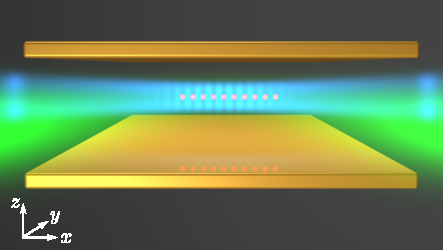
\includegraphics[width=.8\linewidth]{figures/circsim/scheme_simulator}
\caption[Schéma de principe du simulateur quantique]
{Schéma de principe du simulateur quantique proposé.
Les atomes de Rydberg circulaires, représentés par les sphères rouges, sont placés dans un condensateur et piégés dans des faisceaux laser : un faisceau \og creux \fg{} selon l'axe $Ox$, représenté en bleu, et un réseau ajustable créé par l'interférence de deux faisceaux quasi-parallèles, représentés en vert.
Un champ électrique $F$ est imposé entre les deux plaques du condensateur.
}
\label{fig:scheme_simul}
\end{figure}
%
\noindent Le simulateur quantique que nous proposons est schématisé en figure \ref{fig:scheme_simul}.
Une chaîne de spins $1/2$ est simulée par une chaîne d'atomes de Rydberg circulaires.
Les états de spin $\ket{\uparrow}$ et $\ket{\downarrow}$ sont encodés sur les états $\mathrm{50C}$ et $\mathrm{48C}$ respectivement.
L'interaction dipôle-dipôle est alors analogue à un hamiltonien XXZ pour une chaîne de spins $1/2$ en interaction avec leurs plus proches voisins.
Grâce à un champ électrique et à un champ magnétique extérieurs, ainsi qu'à une source microonde couplant les deux niveaux de Rydberg, le hamiltonien simulé peut être contrôlé de façon précise et rapide, sur une large gamme de paramètres.
Cette analogie entre atomes de Rydberg circulaires et spins $1/2$ est établie en \ref{subsec:XXZhamiltonian}, où nous discuterons le choix des niveaux $\mathrm{50C}$ et $\mathrm{48C}$ ainsi que le contrôle du hamiltonien et le diagramme de phase qui en découle.

Les atomes de Rydberg sont piégés par un potentiel laser.
Celui-ci permet un confinement à la fois radial et longitudinal selon l'axe $Ox$.
Le confinement longitudinal étant réalisé par un réseau optique, il présente des pièges périodiquement espacés, et forme ainsi une chaîne unidimensionnelle régulière.
%Des atomes de Rydberg circulaires sont piégés par un potentiel pondéro-moteur créé par des faisceaux laser de longueur d'onde $\lambda = \SI{1064}{\nano\meter}$.
%Le confinement radial sur l'axe $Ox$ est assuré par un faisceau \og creux \fg{} présentant un profil d'intensité de Laguerre-Gauss.
%Le confinement longitudinal est assuré par un réseau unidimensionnel ajustable, formé par l'interférence de deux faisceaux se propageant dans le plan $xOy$, présentant des angles petits et opposés par rapport à l'axe $Oy$.
%La variation de cet angle peut mener à un pas de réseau de $r=\SI{5}{}$ ou $\SI{7}{\um}$ par exemple, ces deux valeurs correspondant respectivement à un régime d'interaction dipôle-dipôle forte ou modérée.
Le principe du piégeage laser des atomes de Rydberg circulaires, ainsi que la géométrie des lasers de piégeage, seront discutés en \ref{subsec:circ_laser_trapping}.

Les atomes de Rydberg circulaires piégés sont placés à l'intérieur d'un condensateur formé par deux électrodes planes parallèles au plan $xOy$.
En plus de permettre l'imposition d'un champ électrique dirigé selon $Oz$, cela inhibe l'émission spontanée $\sigma^+$ du niveau circulaire $\mathrm{nC}$ vers le niveau circulaire $\mathrm{(n-1)C}$.
Comme nous l'avons vu en \ref{subsec:level_50C}, ce canal d'émission est largement responsable de la durée de vie finie des niveaux circulaires.
L'inhibition de ce canal par le condensateur permettra d'accroître significativement la durée de vie des niveaux de Rydberg, jusqu'à des temps de l'ordre de la centaine de secondes.
Le temps de vie des atomes circulaires dans un tel condensateur sera discuté en \ref{subsec:inhibition}.
%Le condensateur permet en second lieu, d'imposer un champ électrique statique homogène selon l'axe $Oz$.

Une technique analogue au refroidissement évaporatif, reposant sur les interactions répulsives entre atomes de Rydberg, permet de préparer de façon déterministe une chaîne régulière de plusieurs dizaines d'atomes de Rydberg circulaires.
\`A la fin d'une simulation, les atomes de Rydberg pourront être détectés un par un grâce à cette même technique, qui sera discutée en \ref{subsec:vdW_evap}.

\subsection{Le hamiltonien simulé}\label{subsec:XXZhamiltonian}
\subsubsection*{De la paire d'atomes de Rydberg à la paire de spins}
\noindent L'interaction entre un atome dans le niveau $\mathrm{nC}$ et un atome dans le niveau $\mathrm{n'C}$ s'écrit comme un hamiltonien effectif
\begin{equation}
\label{eq:Veff_nCn'C}
V_{eff}/h = \left(\begin{array}{cc}
C_{\mathrm{nC},\mathrm{n'C}} & A_{\mathrm{nC},\mathrm{n'C}} \\
A_{\mathrm{nC},\mathrm{n'C}} & C_{\mathrm{nC},\mathrm{n'C}},
\end{array} \right)
\end{equation}
où $C_{\mathrm{nC},\mathrm{n'C}}$ et $A_{\mathrm{nC},\mathrm{n'C}}$ sont respectivement les termes d'interaction directe et d'échange entre les niveaux $\mathrm{nC}$ et $\mathrm{n'C}$.

Étant donné que nous souhaitons simuler une chaîne de spins $1/2$, il nous faut étendre la base des états accessibles.
L'état d'un spin $1/2$ est décrit sur la base $\{\ket{\uparrow},\ket{\downarrow}\}$ et l'état d'une paire de spins $1/2$ est décrit sur la base $\{ \ket{\uparrow \uparrow},\ket{\uparrow \downarrow}, \ket{\downarrow\uparrow}, \ket{\downarrow\downarrow} \}$.
Ainsi en encodant le spin sur des états de Rydberg circulaires par l'équivalence $\ket{\uparrow} = \ket{\mathrm{nC}} , \ket{\downarrow} = \ket{\mathrm{n'C}}$, le hamiltonien d'interaction de la paire de spin doit être étendu à la base 
$\{ \ket{\mathrm{nC},\mathrm{nC}},\ket{\mathrm{nC},\mathrm{n'C}}, \ket{\mathrm{n'C},\mathrm{nC}}, \ket{\mathrm{n'C},\mathrm{n'C}} \}$.
Sur cette base, le hamiltonien d'interaction prend la forme
\begin{equation}
\label{eq:V_eff_nCnC_n'Cn'c}
\hat{V}_{eff}/h = \bordermatrix{
~ 	&\ket{\mathrm{nC},\mathrm{nC}} 	&\ket{\mathrm{nC},\mathrm{n'C}} 
&\ket{\mathrm{n'C},\mathrm{nC}} &\ket{\mathrm{n'C},\mathrm{n'C}} \cr
	\bra{\mathrm{nC},\mathrm{nC}}	& C_{\mathrm{nC},\mathrm{nC}} & 0 & 0 & 0 \cr 
	\bra{\mathrm{nC},\mathrm{n'C}} 	& 0 & C_{\mathrm{nC},\mathrm{n'C}} & A_{\mathrm{nC},\mathrm{n'C}} & 0 \cr
	\bra{\mathrm{n'C},\mathrm{nC}} 	& 0 & A_{\mathrm{nC},\mathrm{n'C}} & C_{\mathrm{nC},\mathrm{n'C}} & 0 \cr
	\bra{\mathrm{n'C},\mathrm{n'C}} & 0 & 0 &  0	& C_{\mathrm{n'C},\mathrm{n'C}}\cr
	}
\end{equation}


Nous souhaitons écrire ce hamiltonien sur la base des opérateurs de spin.
Pour chacun des spins, ces opérateurs sont décrits sur la base de l'identité et des matrices de Pauli $\{\mathbbm{1},\sigma^\alpha \}_{\alpha=x,y,z}$.
Afin d'agir sur l'espace produit tensoriel de deux spins, il nous faut définir les opérateurs suivants
\begin{equation}
\label{eq:Pauli_tensor_space}
\begin{aligned}
\sigma_1^\alpha &= \sigma^\alpha \otimes \mathbbm{1} \\
\sigma_2^\alpha &= \mathbbm{1} \otimes \sigma^\alpha
\end{aligned},
\end{equation}
où l'indice $1$ ou $2$ indique sur quel atome agit l'opérateur.
La famille formée par les produits matriciels deux à deux de ces opérateurs $\mathbbm{1}$\footnote{
Nous omettons délibérément la dimension de l'espace sur lequel agit l'opérateur d'identité. Celui-ci devrait en toute rigueur s'écrire $\mathbbm{1}\otimes \mathbbm{1} = \mathbbm{1}^{\otimes 2}$.
} et $\sigma_i^\alpha$ permet de générer tous les opérateurs agissant sur la paire de spins.
Nous pouvons ainsi réécrire le hamiltonien d'interaction \eqref{eq:V_eff_nCnC_n'Cn'c} sous la forme
%
\begin{equation}
\label{eq:Veff_2at_Pauli}
\begin{aligned}
\hat{V}_{eff}/h &= \delta E~\mathbbm{1}
+ \frac{\delta\zeta}{2}\left( \sigma_1^z + \sigma_2^z \right)
+ J_z\left( \sigma_1^z \sigma_2^z \right)
+ J \left( \sigma_1^x \sigma_2^x + \sigma_1^y \sigma_2^y \right) \\
&= \left( \begin{array}{cccc}
\delta E + \delta \zeta + J_z & 0 & 0 & 0 \\
0 & \delta E - J_z & 2J & 0 \\
0 & 2J & \delta E - J_z & 0 \\
0 & 0 & 0 & \delta E - \delta \zeta + J_z \\
\end{array} \right),
\end{aligned}
\end{equation}
%
où l'on identifie :
%
\begin{equation}
\label{eq:ident_XXZ}
\left\{
\begin{aligned}
\delta E &= \left( \CnCnC + 2\CnCnpC + \CnpCnpC \right)/4, \\
\delta \zeta &= \left( \CnCnC - \CnpCnpC \right)/2, \\
J_z &= \left( \CnCnC - 2\CnCnpC + \CnpCnpC \right)/4, \\
J &= \AnCnpC /2~.
\end{aligned} \right.
\end{equation}
%
Notons que le terme $\delta E \mathbbm{1}$ ne fait que redéfinir l'origine des énergies, et peut donc être ignoré.
Le hamiltonien d'interaction de la paire devient ainsi
\begin{equation}
\label{eq:XXZint_2atoms}
\hat{V}_{eff,\text{2 atomes}}/h = \frac{\delta\zeta}{2}\left( \sigma_1^z + \sigma_2^z \right)
+ J_z\left( \sigma_1^z \sigma_2^z \right)
+ J \left( \sigma_1^x \sigma_2^x + \sigma_1^y \sigma_2^y \right).
\end{equation}
%connu comme \og hamiltonien XXZ \fg{}.

	\subsubsection*{Extension à une chaîne de $N$ atomes et habillage microonde}
\noindent Le hamiltonien d'interaction à deux atomes s'étend facilement à une chaîne de $N$ atomes régulièrement espacés d'une distance $d$ et numérotés de $1$ à $N$.
Nous pouvons ici négliger les interactions au-delà du premier voisin.
En effet, dès lors que les termes d'interaction évoluent en $1/d^6$, la contribution d'un second voisin est $\SI{64}{}$ fois plus petite que celle des premiers voisins.
Le hamiltonien d'interaction d'une telle chaîne de spin s'écrit alors, en généralisant le hamiltonien à deux atomes \eqref{eq:XXZint_2atoms},
%
\begin{equation}
\label{eq:XXZint_Natoms}
\hat{V}_{eff,\text{N}}/h =
\frac{\delta\zeta}{2} \left( \sigma_1^z + \sigma_N^z \right)
+ \delta\zeta \sum_{i=2}^{N-1} \sigma_i^z
+ J_z \sum_{i=1}^{N-1} \sigma_i^z \sigma_{i+1}^z
+ J \sum_{i=1}^{N-1} \left( \sigma_i^x \sigma_{i+1}^x + \sigma_i^y \sigma_{i+1}^y \right) ,
\end{equation}
%
où les opérateurs de spin $\sigma_i^\alpha$ agissant sur l'atome $i$ sont définis par
%
\begin{equation}
\label{eq:Pauli_Natoms}
\sigma_i^\alpha = \overset{\substack{1\\ \downarrow \\}}{\mathbbm{1}}
\otimes\dots\otimes \overset{\substack{i\\ \downarrow \\}}{\sigma^\alpha}
\otimes\dots\otimes \overset{\substack{N\\ \downarrow \\}}{\mathbbm{1}}.
\end{equation}
%
Le premier terme du hamiltonien \eqref{eq:XXZ_Natoms} provient d'un effet de bord :
les atomes à chaque bout de la chaîne n'ont chacun qu'un seul voisin, cependant que les autres atomes en ont chacun deux.
L'énergie d'interaction des atomes $1$ et $N$ est donc deux fois inférieure à celle des atomes du \og c\oe ur \fg{} de la chaîne, numérotés de $2$ à $N-1$.

Le hamiltonien d'interaction \eqref{eq:XXZint_Natoms} ne décrit que l'interaction dipôle-dipôle entre ces atomes.
Or l'évolution de la chaîne de spin dépend également du hamiltonien libre $\hat{H}_0$ de chaque atome, qui induit une différence d'énergie $h\nu_0$ entre les niveaux $\ket{\mathrm{nC}}=\ket{\uparrow}$ et $\ket{\mathrm{n'C}}=\ket{\downarrow}$.
Cette contribution s'écrit sous la forme d'un hamiltonien libre à $N$ atomes $\hat{H}_{0,N}/h = \frac{\nu_0}{2} \sum_{i=1}^{N}\sigma_i^z$.
L'écart d'énergie $h\nu_0$ étant très grand par rapport aux termes d'interaction, nous introduisons 
%De plus, 
un champ microonde afin de coupler les deux niveaux atomiques, 
avec une pulsation de Rabi $\Omega$ et un désaccord $\delta\nu$ par rapport à la transition.
En se plaçant dans le référentiel tournant à la fréquence du champ microonde et sous l'approximation séculaire, un atome isolé évolue selon le hamiltonien 
%ce champ microonde agit sur chaque atome par le hamiltonien
$\hat{H}_{\mu o}/h = \frac{\Omega}{2}\sigma_i^x + \frac{\delta\nu}{2} \sigma_i^z$.

Cette évolution due à l'énergie atomique et au couplage microonde s'ajoute au hamiltonien d'interaction, et nous aboutissons à un hamiltonien total
%
\begin{equation}
\label{eq:hamilt_tot_N}
\begin{aligned}
\hat{H}/h =& %\hat{H}_{0,N}/h + 
\hat{H}_{\mu o,N}/h + \hat{V}_{eff,N}/h \\
=&
%\frac{\nu_0}{2} \sum_{i=1}^{N}\sigma_i^z +
\frac{\Omega}{2}\sum_{i=1}^{N}\sigma_i^x +
\frac{\delta\nu}{2}\sum_{i=1}^{N}\sigma_i^z 
+\frac{\delta\zeta}{2} \left( \sigma_1^z + \sigma_N^z \right)
+ \delta\zeta \sum_{i=2}^{N-1} \sigma_i^z \\
&+ J_z \sum_{i=1}^{N-1} \sigma_i^z \sigma_{i+1}^z
+ J \sum_{i=1}^{N-1} \left( \sigma_i^x \sigma_{i+1}^x + \sigma_i^y \sigma_{i+1}^y \right).
\end{aligned}
\end{equation}
%
La factorisation de cette expression amène finalement au hamiltonien \og XXZ \fg{} d'une chaîne de spins couplés :
\begin{equation}
\label{eq:XXZ_Natoms}
\begin{aligned}
\hat{H}_{\text{XXZ,N}} =
J\cdot & \left[
\sum_{i=1}^{N-1} \left( \sigma_i^x\sigma_{i+1}^x 
+ \sigma_i^y \sigma_{i+1}^y
+ \frac{J_z}{J} \sigma_i^z\sigma_{i+1}^z \right) \right. \\
&\left. + \frac{\Delta}{2J}\sum_{i=1}^{N} \sigma_i^z
+ \frac{\Omega}{2J}\sum_{i=1}^{N} \sigma_i^x \right]
- \frac{\delta\zeta}{2}\left( \sigma_1^z + \sigma_N^z \right),
\end{aligned}
\end{equation}
où $\Delta=\delta\nu+\delta\zeta$.
Sous cette forme, le couplage transverse entre les spins de la chaîne est réglé par le paramètre $J$ et le couplage longitudinal par le paramètre $J_z$.
Le paramètre d'anisotropie du couplage est donné directement par le rapport $J_z/J$.
Le couplage microonde entre les niveaux atomiques est équivalent, pour des spins, à la présence d'un champ magnétique externe.
La composante longitudinale de ce \og champ \fg{} est représentée par le terme $\Delta/(2J)$ et sa composante transverse par le terme $\Omega/(2J)$.
Le dernier terme du hamiltonien représente l'effet de bord de la chaîne évoqué plus haut, qui déplace l'énergie des atomes à chaque bout de la chaîne.

Les paramètres permettant l'exploration de différents régimes d'interaction et d'évolution de la chaîne se réduisent en fin de compte aux trois rapports $J_z/J$, $\Omega/J$ et $\Delta/J$.
Le paramètre $J$, qui rend compte de l'interaction d'échange, règle quant à lui le temps caractéristique d'évolution de la chaîne.
Ce temps est donné par $\tau_{\text{\'ech}} = 1/(4J)$.

	\subsection*{Contrôle du hamiltonien et choix des niveaux 50C et 48C}
\noindent Le niveau de contrôle du hamiltonien \eqref{eq:XXZ_Natoms} est limité par la gamme accessible au rapport $J_z/J$.
Les rapports $\Omega/J$ et $\Delta/J$ sont en effet facilement contrôlables en variant respectivement la puissance et la fréquence du champ microonde utilisé, alors que $J_z/J$ dépend des niveaux atomiques choisis et des champs électrique et magnétique extérieurs que l'on impose aux atomes.
Nous souhaitons que les termes $J_z$ et $J$ soient de même ordre de grandeur, la compétition de ces deux termes ouvrant de larges possibilités d'exploration.
Dans le cas contraire, la dynamique serait largement dominée soit par l'interaction directe soit par l'interaction d'échange, limitant par là la portée du simulateur.

Le rapport $J_z/J$ dépend tout particulièrement de la différence de nombre quantique principal entre les deux niveaux atomiques choisis.
La dépendance des termes d'échange et d'interaction directe en fonction des niveaux atomiques est discutée en détail dans la thèse de Thanh Long Nugyen \cite{PHD_NGUYEN}.
Les calculs d'interaction montrent que pour une paire $\ket{\mathrm{nC},\mathrm{n'C}}$, 
le choix $|n-n'|=2$ nous est favorable : il permet d'obtenir des termes d'échange et d'interaction directe qui sont comparables et évoluent tous deux en $1/r^6$.
Au contraire, pour $|n-n'|=1$, le terme d'échange est très grand et varie en $1/r^3$.
On se trouve alors dans une situation où $J_z/J$ est toujours petit devant $1$ et dépend de la distance inter-atomique.
% et où, de plus, les interactions évoluent souvent en $1/r^3$.
%De plus, une forte interaction d'échange a pour conséquence l'apparition d'une branche attractive forte, comme évoqué en \ref{subsec:inter_60Snl}.
Lorsque $|n-n'|>2$ alors le terme d'échange devient vite négligeable et $J_z/J$ est toujours grand devant $1$.
On se trouve alors dans une situation quasi-classique où l'interaction entre les particules se limite à un déplacement d'énergie répulsif.
%Enfin, la situation $|n-n'|=2$ permet d'obtenir des termes d'échange et d'interaction directe qui sont comparables et évoluent tous deux en $1/r^6$.

Lorsque l'on fait varier le champ électrique $F$ imposé aux atomes, l'effet Stark déplace les niveaux atomiques les uns par rapport aux autres.
Or les termes d'interaction dipôle-dipôle, calculés comme une perturbation de second ordre des énergies, varient comme l'inverse des distances en énergie entre les niveaux.
En changeant ces distances, une variation de $F$ peut avoir un effet important sur les termes d'interaction.
En particulier, $J_z$ est une différence de différents termes d'interaction directe (cf équation \eqref{eq:ident_XXZ}).
Si les termes de cette différence sont suffisamment proches, alors une petite variation de champ électrique peut faite varier grandement $J_z$. %, et même le faire changer de signe.
Le terme $J$, au contraire, est directement proportionnel au terme d'interaction d'échange entre les deux niveaux atomiques.
Sa variation avec $F$ sera donc beaucoup moins forte que celle de $J_z$.
Le champ magnétique a un effet similaire : en déplaçant les énergies des niveaux atomiques par effet Zeeman, il fait varier les coefficients d'interaction.

Le rapport $J_z/J$ ne dépend pas que de la différence $|n-n'|$, mais aussi du nombre quantique principal $n$ lui-même.
En effet, les termes d'interaction directe et d'échange entre les niveaux $\ket{\mathrm{nC}}$ et $\ket{\mathrm{(n-2)C}}$ ne varient pas de la même façon avec $n$.
Le choix $n=50,n'=48$ permet de se situer dans un domaine propice à la flexibilité du simulateur, où $J_z$ et $J$ sont comparables, tout en laissant la possibilité de contrôler la valeur de $J_z/J$ en faisant varier les champs électrique et magnétique extérieurs.
En particulier, les termes d'interaction directe sont suffisamment proches pour permettre un passage par zéro du terme de couplage $J_z$.
La figure \eqref{fig:Jz_Jscan} représente les valeurs accessibles de $J_z/J$ pour les niveaux $\ket{\mathrm{50C}}$ et $\ket{\mathrm{48C}}$, en fonction du champ électrique imposé, pour différents champs magnétiques.
%
\begin{figure}[!h]
\centering
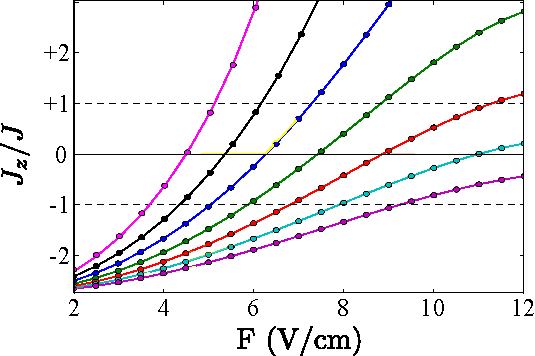
\includegraphics[width=0.7\linewidth]{figures/circsim/Jz_Jscan}
\caption[Variation de $J_z/J$]{
Variation de $J_z/J$ pour une paire d'atomes dans les niveaux $\ket{\mathrm{50C}}$ et $\ket{\mathrm{48C}}$, en fonction du champ électrique $F$.
Le champ électrique est dirigé selon $Oz$ et les atomes sont séparés d'une distance $r=\SI{5}{\um}$ selon l'axe $Ox$.
Les points sont obtenus par diagonalisation du hamiltonien de paire complet pour différentes valeurs de champ magnétique $B_z=\SI{9}{},\SI{10}{},\SI{11}{},\SI{12}{},\SI{13}{},\SI{14}{}$ et $\SI{15}{\gauss}$, de gauche à droite (points de couleur magenta, noir, bleu, vert, rouge, cyan et violet respectivement).
Les lignes qui les relient sont des guides visuels.
}
\label{fig:Jz_Jscan}
\end{figure}
%

Les niveaux atomiques choisis permettent de varier facilement le rapport $J_z/J$ sur une large gamme allant de $-3$ à $+3$, en balayant le champ électrique $F$.
Le contrôle de la source microonde couplant les niveaux atomiques $\mathrm{50C}$ et $\mathrm{48C}$ permet de varier facilement les termes $\Omega$ et $\Delta$ du hamiltonien \eqref{eq:XXZ_Natoms}.
Notons que la variation du terme d'échange $J$ avec les champs électrique et magnétique est très faible alors que le terme d'interaction directe $J_z$, lui, varie beaucoup.
Les trois rapports $J_z/J, \Omega/J$ et $\Delta/J$ sont donc contrôlables de façon quasi-indépendante, puisque $J$ est presque constant.

L'évolution temporelle du système est dominée par le terme d'échange de l'interaction de van der Waals.
Le temps caractéristique d'échange vaut $\tau_{\text{\'ech}} = \SI{14.7}{\us}$ lorsque les atomes sont séparés de $d=\SI{5}{\um}$.
Or le contrôle du champ électrique comme de la source microonde sont rapides, de l'ordre de la centaine de nano-secondes.
Le hamiltonien est ainsi sous contrôle expérimental intégral, à des échelles temporelles très inférieures au temps caractéristique de l'évolution du système.
%, dominé par le terme d'échange dans l'interaction.
%Ce temps d'échange est donné par $\tau_{\text{\'ech}} = 1/(4J) = \SI{14.7}{\us}$ lorsque les atomes sont séparés de $r=\SI{5}{\um}$.% et $\SI{108}{\us}$ si les atomes sont séparés de $r=\SI{7}{\um}$.

Grâce à ce très bon niveau de contrôle du hamiltonien, il est possible d'explorer à volonté le diagramme de phase présenté en figure \eqref{fig:phase_diagram}, extrait des résultats de \cite{MX_DMITRIEV02} et détaillé dans \cite{ENS_PRE_CIRCSIM}.
%
\begin{figure}[!h]
\centering
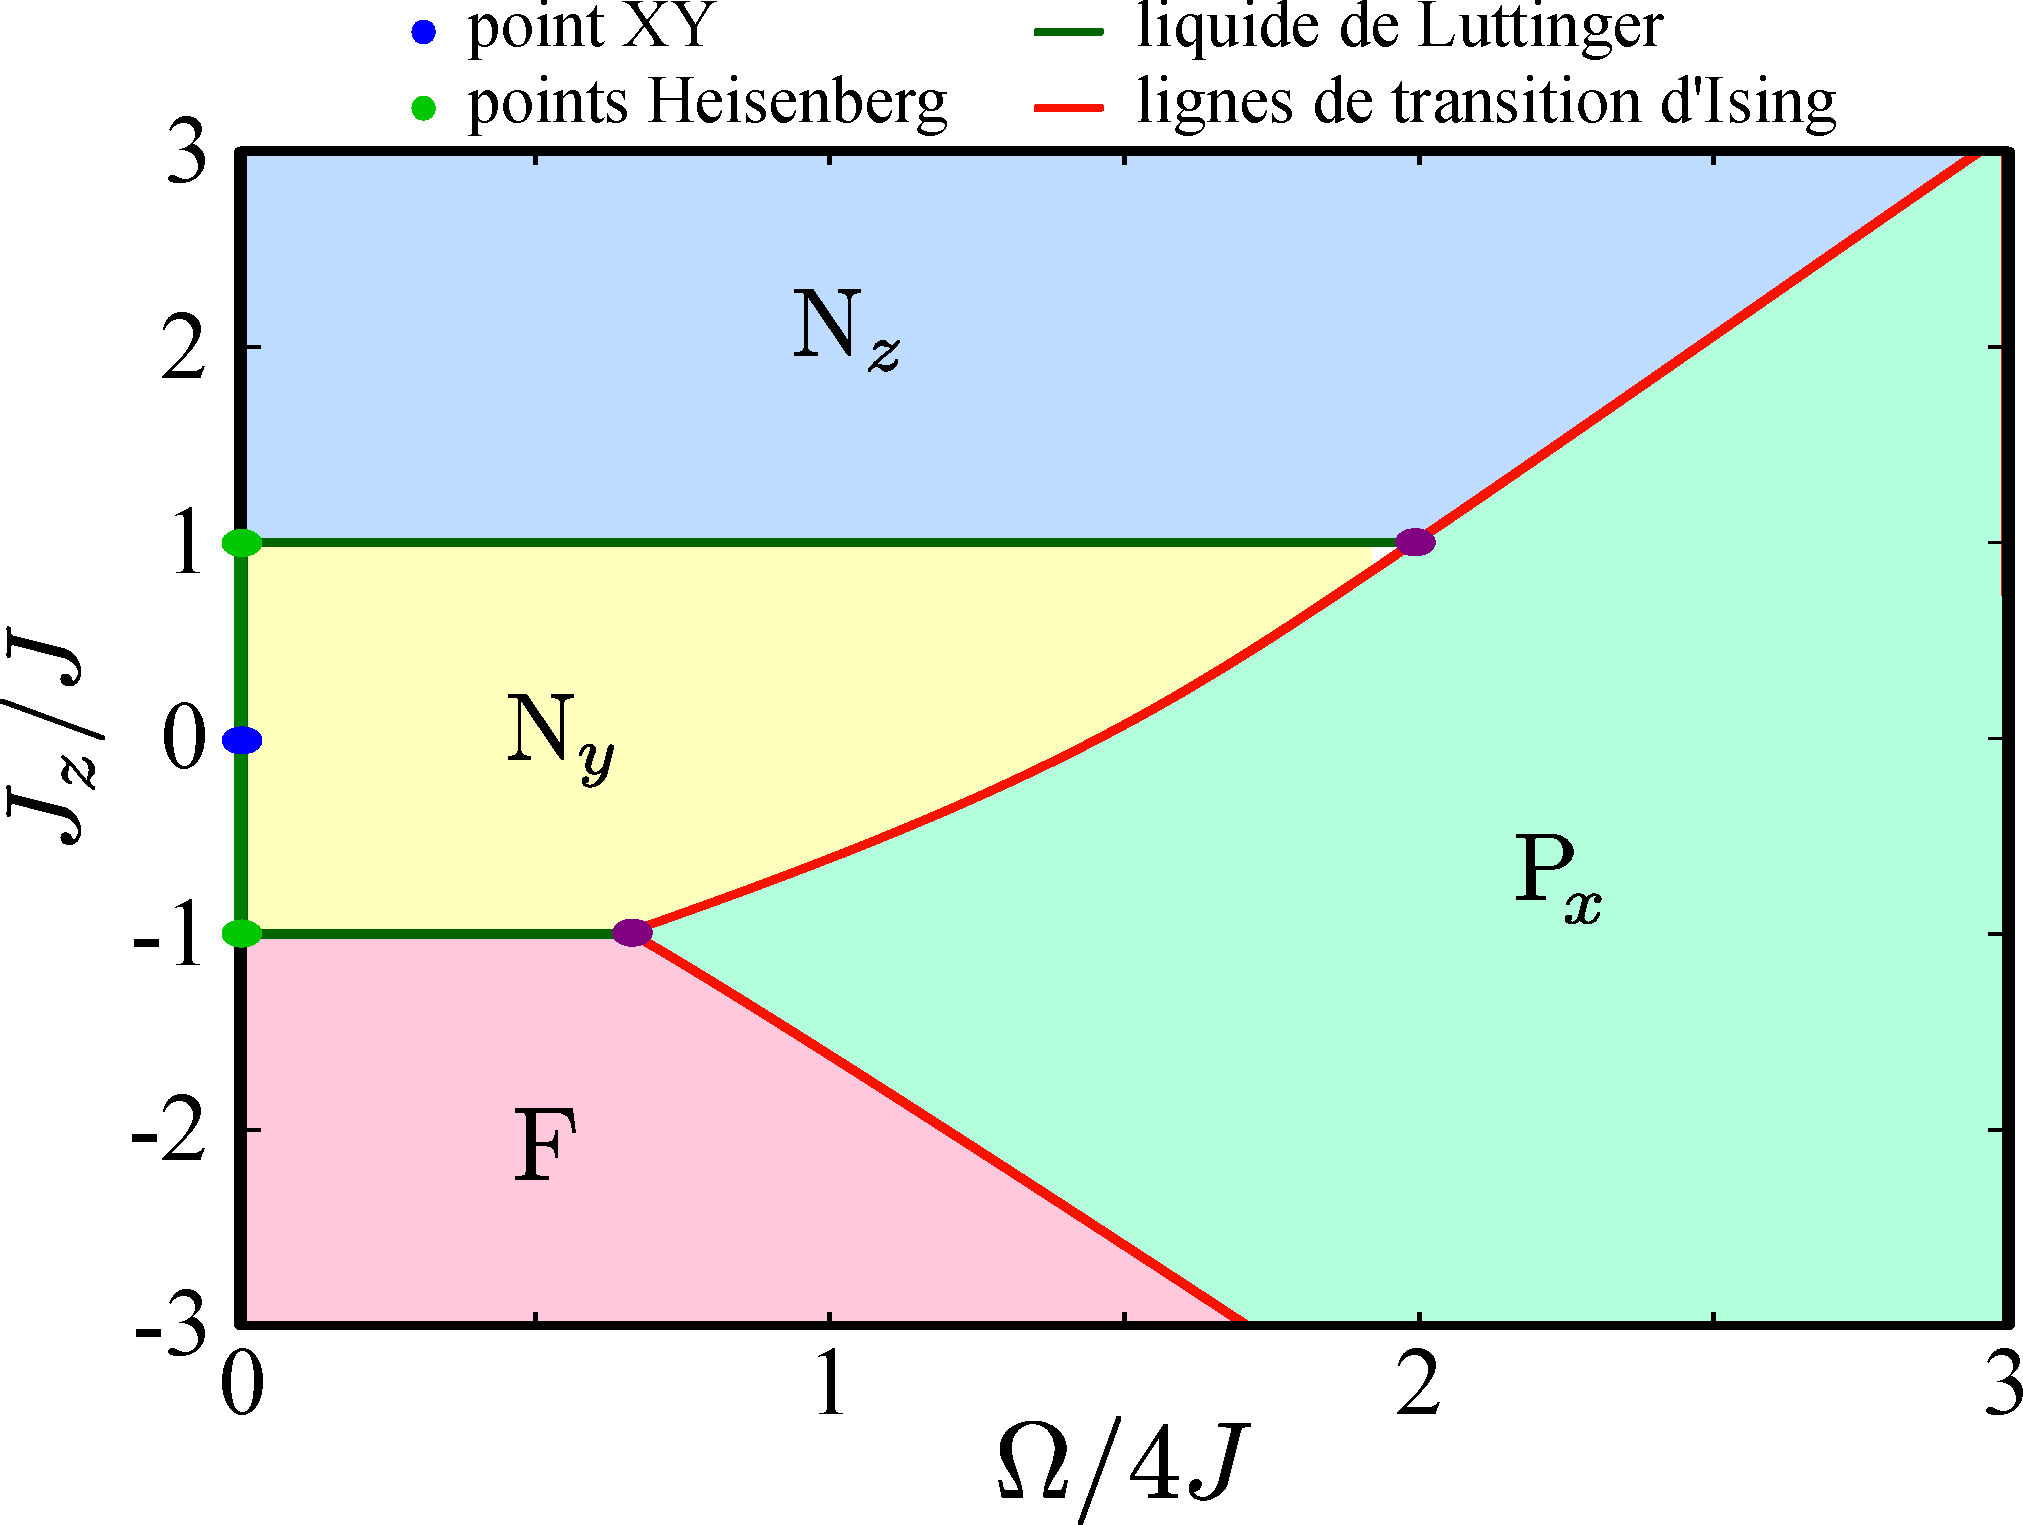
\includegraphics[width=0.7\linewidth]{figures/circsim/phase_diagram}
\caption[Diagramme de phase XXZ]{
Schéma du diagramme de phase du hamiltonien \eqref{eq:XXZ_Natoms} pour $\Delta=0$ et en négligeant le terme d'effet de bord $\delta\zeta$.
Les différentes phases représentées sont : une phase $P_x$ dans laquelle les spins suivent un ordre ferromagnétique selon la direction $x$, une phase $F$ ferromagnétique selon la direction $z$, deux phases de Néel $N_y$ et $N_z$ selon les axes $y$ et $z$ repsectivement.
La phase $P_x$ est séparée des autres par des lignes \og de transition d'Ising \fg{}, le long desquelles le système se réduit au modèle d'Ising.
Le long des frontières entre les phases $N_z$ et $N_y$ et entre les phases $N_y$ et $F$, le système se comporte comme un \og liquide de Luttinger \fg{}, généralisation en présence d'un champ magnétique des \og points de Heisenberg \fg{}.
Le point singulier $XY$ marque la situation où le terme $J_z$ est nul.
}
\label{fig:phase_diagram}
\end{figure}
%
Ce diagramme présente une grande richesse de phases et de transitions de phase.
Une approche statique permettrait de calibrer le simulateur sur des phases connues, puis de simuler une évolution adiabatique passant par des transitions de phase quantiques.
Le rapidité de contrôle du hamiltonien permettrait ensuite de simuler des trempes : des changements de paramètres brusques induisant des états hors-équilibre.

	\subsection{Piégeage laser des atomes de Rydberg circulaires}\label{subsec:circ_laser_trapping}
\noindent Afin de pouvoir observer les atomes de Rydberg en interaction pendant des temps longs, il est nécessaire de les piéger.
Les atomes de Rydberg circulaires peuvent être piégés grâce au potentiel pondéro-moteur créé, pour l'électron de valence, par un faisceau laser.
Cet électron de valence, quasi-libre, se comporte comme une particule chargée dans un champ électrique rapidement oscillant.
Il subit ainsi un déplacement d'énergie positif, proportionnel à l'intensité lumineuse $I_L$ \cite{MX_FABRERYDHF76} :
\begin{equation}
\label{eq:pondero_energy}
\mathcal{E} = \frac{q^2}{2m_e \epsilon_0 c \omega_L^2} I_L
= \frac{h\alpha}{m_e\omega_L^2}I_L,
\end{equation}
où $\omega_L/2\pi$ est la fréquence du laser et $\alpha = q^2/(4\pi\hbar\epsilon_0 c)$ est la constante de structure fine.
Le c\oe ur positif de l'atome de Rydberg subit un déplacement d'énergie négatif $\mathcal{E}_{\text{c\oe ur}} = - h\alpha I_L/(M\omega_l^2)$, où $M$ est la masse du c\oe ur atomique.
Celle-ci étant très grande devant la masse $m_e$ de l'électron, l'effet du laser sur le c\oe ur atomique peut être négligé.
En fin de compte, le potentiel pondéro-moteur \eqref{eq:pondero_energy} agit sur l'atome de Rydberg de sorte que celui-ci recherche les basses intensités lumineuses.

La géométrie que nous cherchons à obtenir est une chaîne unidimensionnelle.
Le confinement radial selon l'axe $Ox$ est assuré par un faisceau \og creux \fg{} de longueur d'onde $\lambda=\SI{1064}{\nano\meter}$, présentant un profil d'intensité de Laguerre-Gauss d'ordre $(0,1)$.
Ce profil d'intensité $LG_0^1$ est proportionnel à $(2\rho^2/w^4)\cdot e^{-2\rho^2/w^2}$, où $\rho$ est la distance à l'axe optique et $w$ le col du faisceau\footnote{
La définition du col pour un profil de Laguerre-Gauss découle directement de celle pour un faisceau gaussien.
}.
La figure (\ref{fig:pondero_trap} a) représente le potentiel créé par ce faisceau dans le plan $x=0$, pour une puissance laser de $\SI{0.5}{\watt}$ focalisée sur un col $w=\SI{7}{\um}$.
Dans ces conditions, les atomes sont piégés transversalement à l'axe $Ox$ avec des fréquences de piégeage $\omega_y=\omega_z= 2\pi\times \SI{12}{\kHz}$.

\begin{figure}[h]
\centering
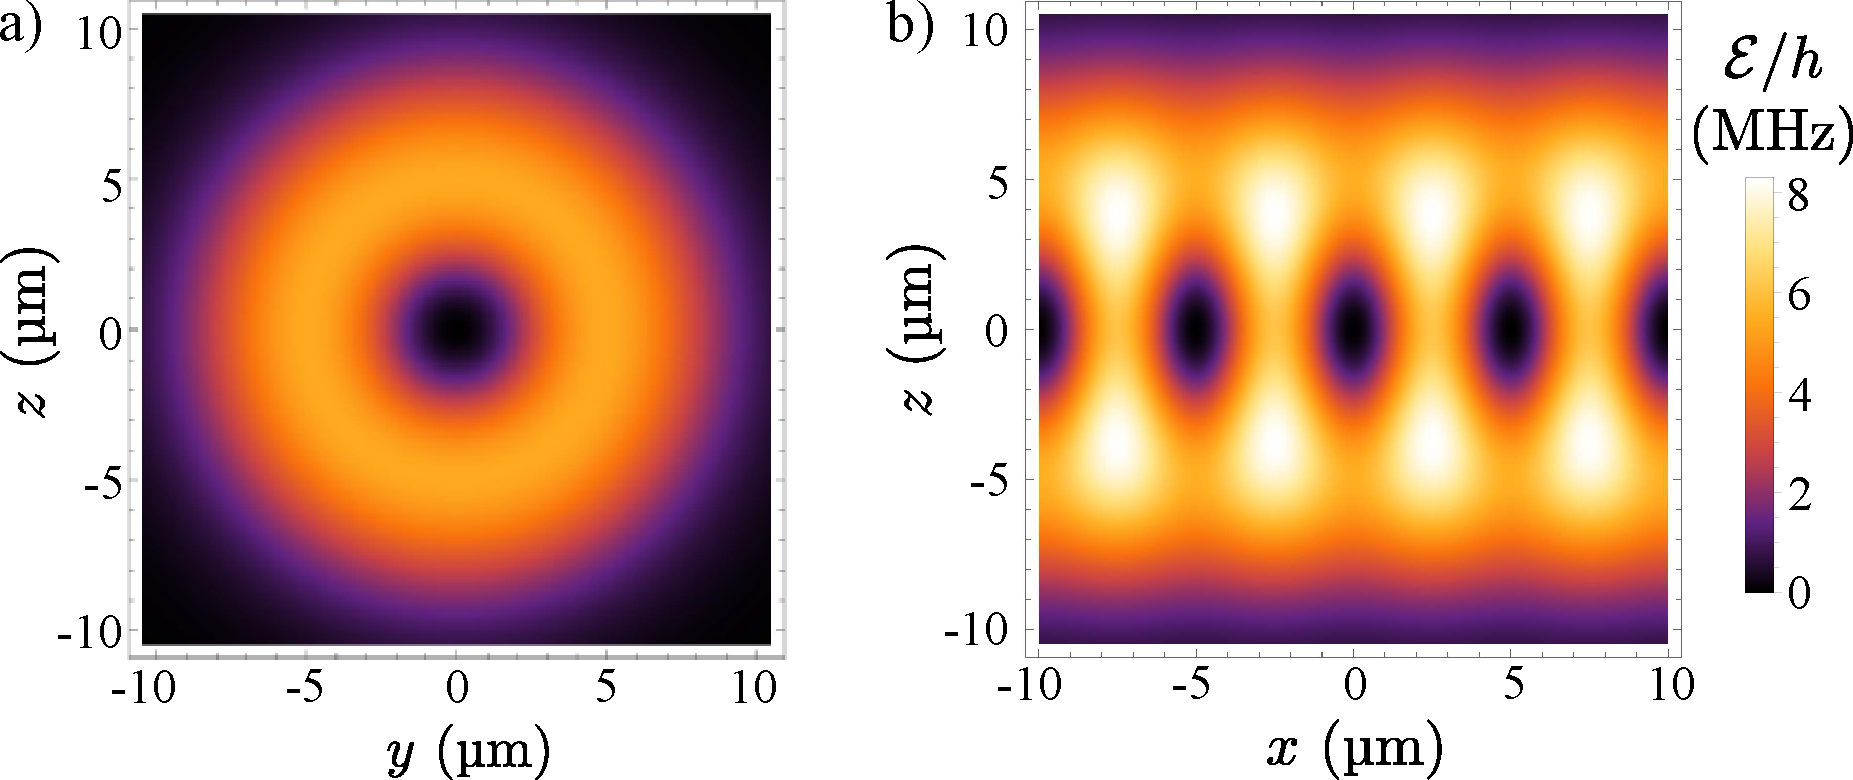
\includegraphics[width=\linewidth]{figures/circsim/pondero_trap}
\caption[Potentiel de piégeage pondéro-moteur]{
\textbf{a)} Coupe dans le plan $yOz$ du potentiel pondéro-moteur créé par le faisceau Laguerre-Gauss se propageant selon l'axe $Ox$.
\textbf{b)} Coupe dans le plan $xOz$ du potentiel de piégeage pondéro-moteur créé par le faisceau Laguerre-Gauss et les deux faisceaux gaussiens en interférence.
Le potentiel est exprimé en unités de fréquence. L'échelle de couleur est commune aux deux graphes.
}
\label{fig:pondero_trap}
\end{figure}
	
Le confinement longitudinal doit permettre de fixer la distance séparant les atomes de la chaîne.
Ce piégeage doit donc être périodique.
En effet, l'interaction de van der Waals répulsive entre atomes de Rydberg entraînerait un mouvement important des atomes le long de l'axe $Ox$ en l'absence de piégeage périodique longitudinal.
Afin de réaliser ce confinement, nous proposons d'utiliser un réseau lumineux d'un pas ajustable de l'ordre de $d=\SI{5}{}$.
Ce réseau est créé par l'interférence à petit angle de deux faisceaux gaussiens.
Ceux-ci sont décalés en fréquence de quelques dizaines de $\SI{}{\MHz}$ par rapport au faisceau Laguerre-Gauss afin de ne pas interférer avec lui.
Les deux faisceaux gaussiens se propagent dans le plan $xOy$ avec un angle $\pm \theta$ par rapport à l'axe $Oy$.
Pour obtenir un pas de réseau de $d=\SI{5}{\um}$, cet angle doit prendre une valeur $\theta=\SI{5.7}{\degree}$.
Ces deux faisceaux gaussiens sont allongés selon l'axe $Ox$ afin que le réseau créé puisse recouvrir toute la longueur de la chaîne atomique.
Ainsi, leur col selon $x$ vaut $w_x = \SI{200}{\um}$ alors que leur col selon $z$ vaut $w_z=\SI{7}{\um}$.
Dans ces conditions, et avec une puissance totale par faisceau de $\SI{1.45}{\watt}$, les atomes sont piégés dans la direction $x$ avec une fréquence $\omega_x = 2\pi \times \SI{24}{\kHz}$ et une profondeur de piège proche de $\SI{4}{\MHz}$, soit environ $\SI{200}{\uK}$.

Le potentiel créé dans le plan $xOz$ par la superposition du faisceau Laguerre-Gauss et de ces deux faisceaux gaussiens est représenté en figure (\ref{fig:pondero_trap} b), pour un pas de réseau de $\SI{5}{\um}$.
Nous disposons ainsi d'une chaîne de pièges profonds régulièrement espacés sur l'axe $Ox$.

	
	\subsection{Préservation des états de Rydberg}\label{subsec:inhibition}
\noindent Le piégeage laser présenté ci-dessus permet de fixer les positions des atomes de Rydberg circulaires au sein d'une chaîne unidimensionnelle.
Si l'on en reste au calcul de \ref{subsec:level_50C}, chaque atome dans le niveau $\mathrm{50C}$ a une durée de vie de $\SI{8.36}{\ms}$ à $\SI{4.2}{\K}$.
Une chaîne de quarante atomes a ainsi une durée de vie de $\SI{8.36}{}/\SI{40}{} = \SI{0.21}{\ms}$.
Avec des atomes séparés de $d=\SI{5}{\um}$ et donc un temps d'échange $\tau_{\text{éch}} = \SI{14.7}{\us}$, la chaîne d'atomes vit le temps d'une quinzaine d'échanges.
C'est-à-dire qu'une excitation placée à un bout de la chaîne n'aurait pas le temps de se propager jusqu'au milieu de la chaîne.
La solution la plus évidente pour rallonger la durée de vie d'un niveau de Rydberg consiste à refroidir l'environnement afin de réduire au mieux l'émission stimulée par le rayonnement du corps noir.
Cependant, cela ne permettrait ici de l'améliorer que d'un facteur $%\SI{8.36}{}/\SI{28.65}{} \simeq 
\SI{3.5}{}$ au maximum, la durée de vie à température nulle étant de $\SI{28.65}{\ms}$ pour le niveau $\mathrm{50C}$.

Comme nous l'avons vu en \ref{subsec:level_50C}, le seul processus limitant la durée de vie à température nulle d'un niveau de Rydberg circulaire $\mathrm{nC}$ est la désexcitation spontanée vers le niveau $\mathrm{(n-1)C}$ par une transition $\sigma^+$.
Inhiber cette transition pourrait ainsi permettre d'augmenter significativement le temps de vie d'un niveau circulaire.
Mais comment inhiber l'émission spontanée ?
L'effet Purcell, observé en 1946 \cite{Purcell46_Purcelleffect}, consiste à augmenter le taux d'émission spontanée en plaçant le système émetteur dans une cavité résonante avec la transition considérée.
Cet effet repose sur l'augmentation des fluctuations du vide électromagnétique dans le mode d'émission.
Au contraire, il s'agit pour nous de réduire le plus possible ces fluctuations afin d'inhiber l'émission.
Pour cela, il suffit que la cavité soit de dimensions plus petites que la longueur d'onde du rayonnement que l'on souhaite inhiber \cite{MX_KELPPNER_INHIBITION,MX_KLEPPNERINHIBITION85}.
Plus, précisément, dans le cas d'un condensateur formé de deux plans parallèles, la distance $D$ entre ces deux plans doit être inférieure à la moitié de la longueur d'onde $\lambda$ du rayonnement :
%
\begin{equation}
\label{eq:condition_inhib}
D< \lambda/2.
\end{equation}
%
L'émission de photons dans la direction normale aux plaques du condensateur peut alors être inhibée sous la condition \eqref{eq:condition_inhib}, alors que l'émission selon une direction parallèle aux plaques ne l'est pas.
Or, lorsque l'on impose un champ électrique entre les deux plaques du condensateur, celui-ci fixe l'axe de quantification du moment cinétique des atomes de Rydberg.
L'émission sur une transition $\sigma^+$ se fait alors nécessairement dans la direction normale aux plaques et peut être inhibée.
%L'émission dans une direction parallèle aux plaques n'est pas inhibée.

Les transitions $\mathrm{50C}\rightarrow \mathrm{49C}$ et $\mathrm{48C}\rightarrow \mathrm{47C}$ ont des fréquences respectives de $\SI{54.249}{\GHz}$ et $\SI{61.407}{\GHz}$, correspondant à des longueurs d'onde de $\SI{5.525}{\mm}$ et $\SI{4.882}{\mm}$.
La condition \eqref{eq:condition_inhib} nous impose donc de placer les atomes de Rydberg circulaires dans un condensateur dont les deux plaques sont distantes de $D<\SI{2.4}{\mm}$.
Dans le cas d'un condensateur infini idéal, cela suffirait à inhiber complètement le rayonnement à ces fréquences, et ainsi à rendre la durée de vie des niveaux circulaires infinie.

En pratique, il est nécessaire de tenir compte de la taille et de la conductivité finies du condensateur dans lequel nous placerons les atomes.
%De plus, en raison de la température finie de l'environnement, quelques photons thermiques sont présents qui peuvent stimuler des transitions $\pi$ depuis un niveau circulaire $\mathrm{nC}$ vers un niveau elliptique $\mathrm{nE^{\pm}}$ de la multiplicité du dessus.
%Ces transitions $\pi$ ne sont malheureusement pas inhibées par le condensateur puisqu'elles ont lieu dans le plan de celui-ci.
Une simulation effectuée avec la suite logicielle CST Studio permet de calculer numériquement le taux d'émission spontanée résiduelle $\Gamma$ des atomes à l'intérieur d'un condensateur formé de deux plaques d'or carrées de côté $a$, refroidies à une température d'$\SI{1}{\K}$ et distantes de $D$.
La figure \eqref{fig:inhibition_factor} représente le rapport $\Gamma/\Gamma_{\mathrm{48C}}$ en fonction de $a$ et $D$, où $\Gamma_{\mathrm{48C}}$ est le taux d'émission spontanée depuis le niveau circulaire $\mathrm{48C}$ dans l'espace libre.
%
\begin{figure}[h]
\centering
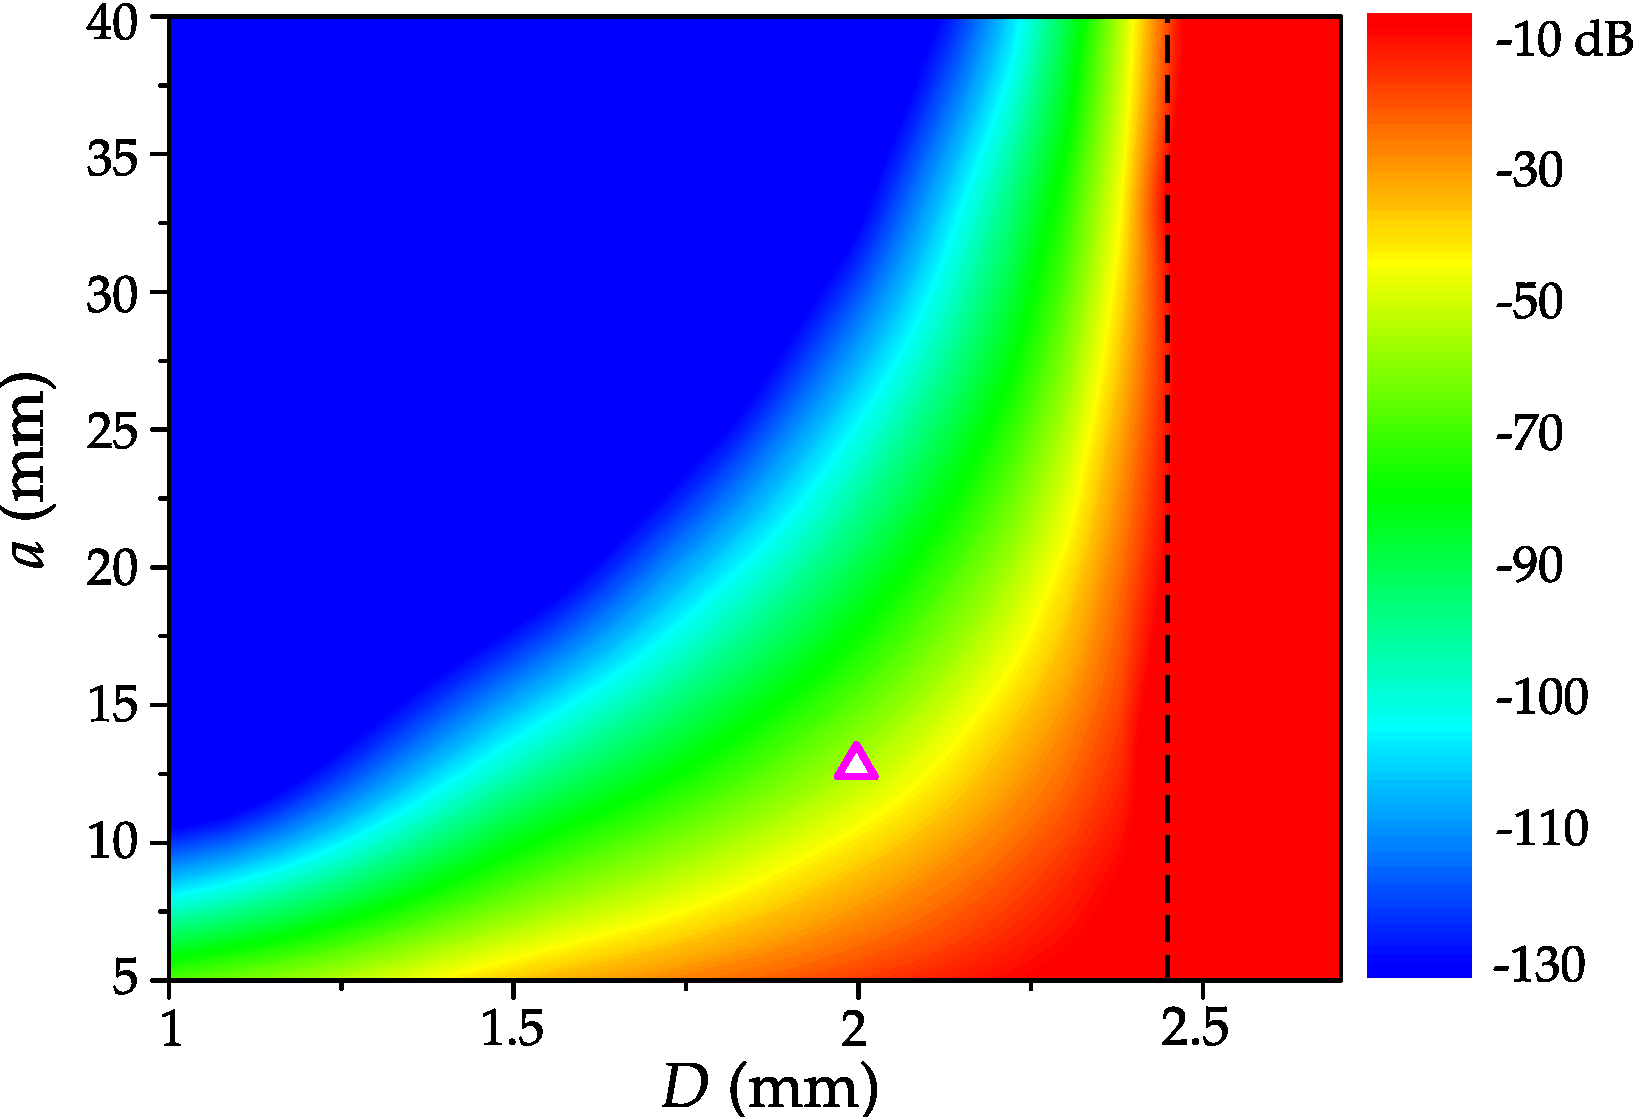
\includegraphics[width=.7\linewidth]{figures/circsim/inhibition_factor}
\caption[Inhibition de l'émission spontanée en fonction des dimensions du condensateur]{
Rapport d'inhibition de l'émission spontanée $\Gamma/\Gamma_{\mathrm{48C}}$ en échelle log, en fonction de l'espacement $D$ et de la taille $a$ du condensateur.
La ligne pointillée se situe à $D=\lambda/2$ et le triangle rouge représente les paramètres choisis $D=\SI{2}{\mm}$ et $a=\SI{13}{\mm}$.
L'émission spontanée y est inhibée de $\SI{50}{\decibel}$.
}
\label{fig:inhibition_factor}
\end{figure}
%
Nous choisissons les paramètres $D=\SI{2}{\mm}$ et $a=\SI{13}{\mm}$, où l'émission spontanée depuis le niveau $\mathrm{48C}$ est inhibée d'un facteur $\SI{50}{\decibel}$.
Cela amène la durée de vie du niveau $\mathrm{48C}$ à environ $\SI{2500}{\second}$.
L'effet d'inhibition est encore meilleur pour le niveau $\mathrm{50C}$ puisque l'émission spontanée depuis celui-ci se fait à une longueur d'onde plus grande.
Nous disposons donc \textit{a priori} d'un temps de vie quasi-infini par rapport aux échelles de temps de l'évolution de la chaîne de spins.

	\subsection{Préparation déterministe d'une chaîne}\label{subsec:vdW_evap}
\noindent À des fins évidentes de reproductibilité, la chaîne de $N$ atomes constituant le simulateur doit être préparée de façon déterministe.
Pour cela, nous proposons une méthode de préparation fondée sur une variante du refroidissement évaporatif.
Une chaîne initiale, irrégulière et contenant un grand nombre aléatoire d'atomes, est comprimée et \og évaporée \fg{} jusqu'à obtenir le nombre d'atomes et la distance inter-atomique souhaités.
Ce processus d'évaporation refroidit les atomes presque jusqu'à l'état fondamental du piège laser.
Cette technique permet également d'obtenir une détection individuelle des atomes de Rydberg.

Une séquence expérimentale typique commence par la préparation d'un nuage thermique de \Rb{87} près d'une puce supraconductrice, très allongé dans la direction $x$ et refroidi à une température inférieure à $\SI{1}{\uK}$, proche de la dégénérescence.
Ce nuage est ensuite piégé dans le potentiel dipolaire, créé par un faisceau laser focalisé, et déplacé vers le condensateur d'inhibition précédemment décrit.
Là, après extinction du piège dipolaire, une impulsion laser à deux photons excite un nuage d'atomes de Rydberg à bas moment cinétique de nombre quantique principal $n=50$, en régime de blocage dipolaire.
En raison de la forme allongée du nuage d'atomes dans l'état fondamental et du blocage dipolaire, cet ensemble d'atomes de Rydberg est une chaîne irrégulière contenant une centaine d'atomes distants de $\SI{9}{}\pm\SI{3}{\um}$.
Les atomes dans l'état fondamental sont expulsés par une impulsion laser résonante à $\SI{780}{\nano\meter}$, et les atomes de Rydberg sont transférés vers l'état circulaire $\mathrm{50C}$ grâce à un champ radio-fréquence polarisé $\sigma^+$\footnote{Le processus de circularisation sera discuté au chapitre \ref{chapter:50c}.}.

Lorsque les atomes de Rydberg circulaires sont excités, le faisceau Laguerre-Gauss de confinement radial est allumé, en même temps que deux faisceaux gaussiens \og bouchons \fg{} parallèles à l'axe $Oy$.
Ces deux faisceaux à $\SI{1064}{\nano\meter}$ créent deux barrières d'énergie sur l'axe $Ox$, centrées en $x=\pm L/2$, représentées en figure (\ref{fig:plugs_evap} a).
Le bouchon de droite ($x=+L/2$) est plus bas en énergie que celui de gauche.
Le piège est ensuite comprimé en réduisant $L$.
Ce faisant, les atomes de Rydberg sont approchés les uns des autres ce qui fait augmenter l'interaction répulsive de van der Waals.
Lorsque la chaîne d'atomes est suffisamment comprimée, l'atome en bout de chaîne à droite a une énergie d'interaction qui devient supérieure à la hauteur de la barrière créée par le bouchon laser, et cet atome est ainsi éjecté de la chaîne, comme cela est représenté en figure (\ref{fig:plugs_evap} b).
Les atomes restants se redistribuent selon l'axe $x$ et l'énergie totale de la chaîne se trouve diminuée par cette \og évaporation \fg{} d'un atome.
Le nombre final d'atomes dans la chaîne est déterminé par la valeur finale de $L$ et par la hauteur en énergie du bouchon laser.
%
\begin{figure}[h]
\centering
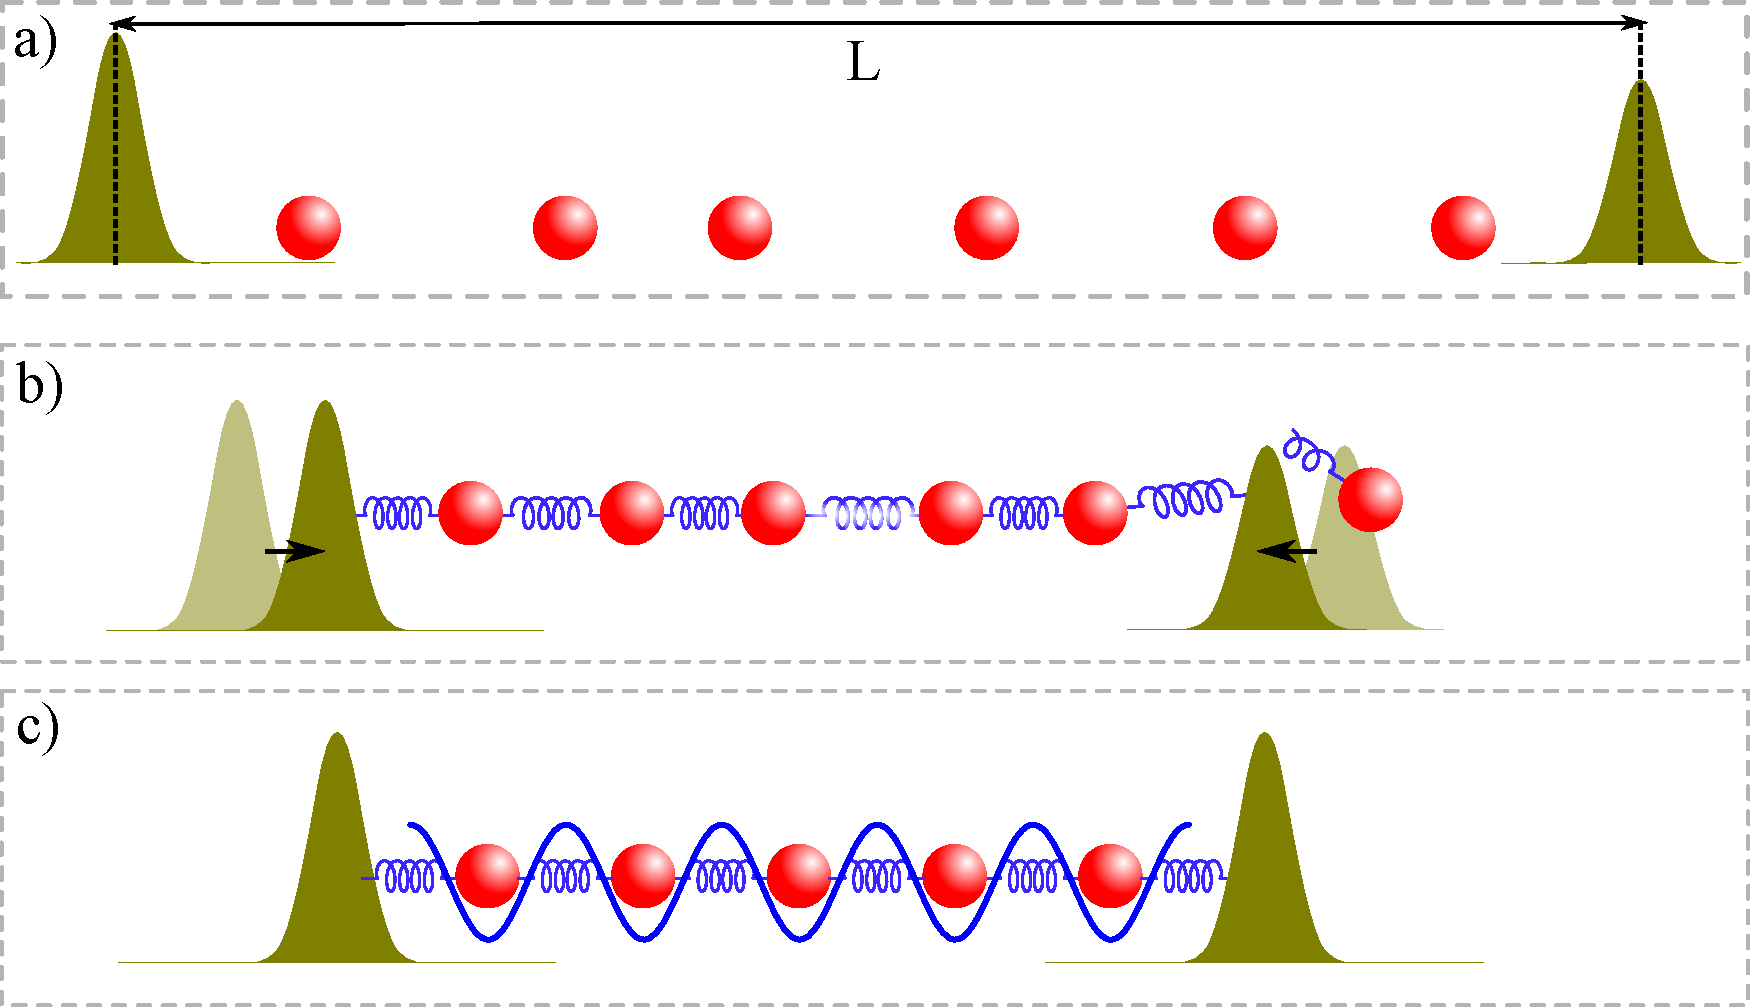
\includegraphics[width=0.8\linewidth]{figures/circsim/plugs_evap}
\caption[Schéma de l'\og évaporation van der Waals \fg{} ]{
Schéma de l'\og évaporation van der Waals \fg{}.
\textbf{a)} Une chaîne irrégulière est préparée et piégée entre deux \og bouchons \fg{} laser séparés d'une distance $L$.
\textbf{b)} En diminuant $L$, on augmente les interactions de van der Waals répulsives entre les atomes de la chaîne.
La barrière énergétique étant plus basse à droite, l'atome au bout de la chaîne est éjecté.
\textbf{c)} \`A la fin du processus d'évaporation, on obtient de façon déterministe une chaîne régulière de $N$ atomes. Un réseau laser est allumé afin de piéger chaque atome.
}
\label{fig:plugs_evap}
\end{figure}
%

Ce processus de refroidissement évaporatif peut être simulé numériquement de façon quasi-classique.
La figure \eqref{fig:nevap} présente le résultat de $\SI{100}{}$ réalisations de la séquence d'évaporation, en moyenne et variance du nombre d'atomes final en fonction de la valeur finale de $L$.
Pour les nombres d'atomes inférieurs à $\SI{45}{}$, $N$ évolue par des pas bien définis, et l'insert qui détaille les résultats autour de $N=40$ montre l'annulation de la variance du nombre d'atomes à certaines valeurs de $L$.
En arrêtant à ces longueurs de piège le processus d'évaporation, nous obtenons de façon déterministe une chaîne avec le nombre d'atomes voulu.
La distance inter-atomique $d$ est ensuite choisie par un ajustement fin de la longueur $L$.
%
\begin{figure}[h]
\centering
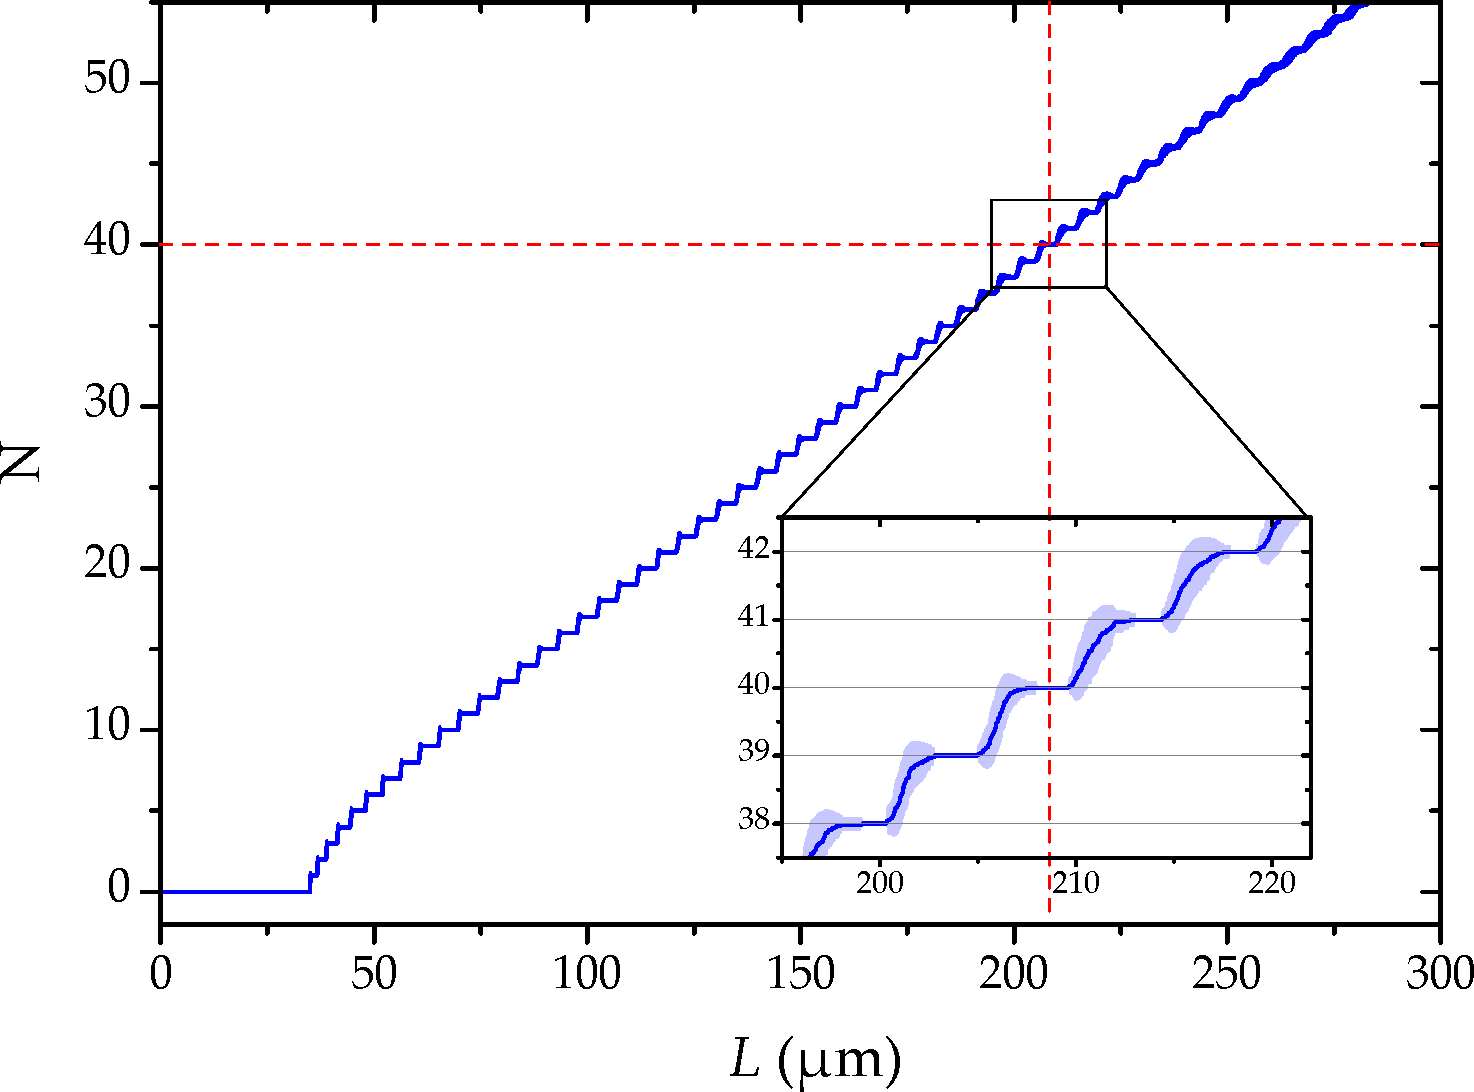
\includegraphics[width=0.6\linewidth]{figures/circsim/nevap}
\caption[Nombre d'atomes restant après évaporation van der Waals]{
Nombre d'atomes $N$ restant après l'évaporation van der Waals, en fonction de la valeur finale de la distance $L$ entre les deux bouchons laser.
Le trait plein représente la moyenne de $N$ sur $100$ réalisations du processus d'évaporation.
La variance de $N$ est indiquée par les zones bleu clair.

}
\label{fig:nevap}
\end{figure}
%

Enfin, le réseau laser de confinement longitudinal est allumé adiabatiquement afin de fixer les positions atomiques.
Les faisceaux bouchons sont gardés allumés, avec une puissance ajustée de façon à compenser la répulsion des atomes du bout de la chaîne par leur unique voisin.
L'état final de la chaîne d'atomes est représenté en figure (\ref{fig:plugs_evap} c).

La procédure d'évaporation peut également servir à la détection des atomes de Rydberg.
\`A la fin de l'évolution de la chaîne de spins, une impulsion $\pi$ microonde est appliquée sur la transition $\mathrm{48C}\rightarrow\mathrm{46C}$.
Si elle présente une fréquence de Rabi suffisante, cette impulsion assure le transfert vers le niveau $\mathrm{46C}$ de tous les atomes dans le niveau $\mathrm{48C}$, quelle que soit leur énergie d'interaction.
L'interaction d'échange entre $\mathrm{50C}-\mathrm{46C}$ étant de l'ordre du $\SI{}{\milli\hertz}$, ce transfert arrête l'évolution de la chaîne de spins et \og gèle \fg{} les états de spin.
Le réseau de confinement longitudinal est alors éteint, et le processus d'évaporation par compression de la chaîne peut reprendre.
Chaque atome est ainsi tour à tour expulsé de la chaîne et guidé par le faisceau Laguerre-Gauss vers une zone de détection située en-dehors du condensateur d'inhibition.
Ils sont détectés dans cette zone par ionisation, ce qui projette leur état sur la base $\{\ket{\mathrm{46C}},\ket{\mathrm{50C}}\}$, équivalente à la base $\{\ket{\uparrow},\ket{\downarrow} \}$.
Grâce à une impulsion microonde supplémentaire, appliquée juste avant le gel des interactions, nous pouvons imposer une rotation arbitraire aux états de spin. Ainsi nous pouvons mesurer toute observable de spin souhaitée, la seule contrainte étant que cette observable doit être la même pour tous les atomes de la chaîne.
En fin de compte, l'état de chaque spin peut être individuellement mesuré en fonction du temps selon n'importe quelle observable.
Cela permet d'accéder à des fonctions de corrélations complexes et aux propriétés d'intrication de la chaîne de spins.

\section{Le mélange des niveaux de paire entre atomes de Rydberg circulaires}
\noindent Les interactions dipôle-dipôle entre atomes de Rydberg circulaires sont au c\oe ur de notre proposition de simulateur.
Or, comme nous l'avions évoqué en \ref{subsec:interac50C_I}, les interactions entre atomes de Rydberg circulaires sont compliquées par le mélange des niveaux de paires atomiques avec des niveaux de paire voisins.
Dans notre exemple du chapitre \ref{chapter:Rydberg}, cela se produisait pour une paire d'atomes dans le niveau $\mathrm{50C}$ dans un champ électrique de $\SI{1}{\V/\cm}$, dès que la distance inter-atomique étaient inférieure à $\SI{10}{\um}$.

Ce problème de mélange des niveaux a deux effets principaux en ce qui nous concerne.
Tout d'abord, les interactions dipôle-dipôle en dépendent fortement.
De plus, les transitions de désexcitation des niveaux elliptiques ne sont pas toutes inhibées par le condensateur dans lequel nous souhaitons placer les atomes.
Le mélange des niveaux atomiques aura donc une incidence importante sur le temps de vie de la chaîne.

Après avoir présenté plus en détail ce problème du mélange des niveaux et indiqué comment le limiter par l'introduction d'un champ magnétique extérieur, nous évaluerons son influence, ainsi que celle d'autres facteurs secondaires, sur le temps de vie des atomes de Rydberg circulaires dans le condensateur. 

\subsection{Interactions dipôle-dipôle entre atomes de Rydberg circulaires : mélange de niveaux}
\label{subsec:circ_interactions}

\noindent Les atomes de Rydberg de grand moment cinétique nécessitent un champ électrique extérieur afin de fixer un axe de quantification, et donc de fixer l'orientation des orbites électroniques.
Dans la présente discussion, nous considérerons que les atomes de Rydberg circulaires sont placés sur un axe $Ox$, perpendiculaire au champ directeur selon $Oz$, tels que représentés en figure \eqref{fig:scheme_simul}.

%\subsubsection{Les niveaux circulaires en présence de champs électrique et magnétique}%\label{subsec:circulars_in_fieds}
%\noindent 
En présence d'un champ électrique, les niveaux à grand moment cinétique d'une même multiplicité voient leur dégénérescence partiellement levée.
Le diagramme d'énergie de ces niveaux est représenté en figure (\ref{fig:ener_StarknC_nCnC}a)).
Le niveau circulaire est noté $\ket{\mathrm{nC}}$ et les deux niveaux \og elliptiques \fg{} voisins sont notés $\ket{\mathrm{nE^{\pm}}} = \ket{n,m=n-2,k=\pm1}$.
De la même façon, les niveaux de $m=n-3$ sont notés $\ket{\mathrm{nEE^0}} = \ket{n,m=n-3,k=0}$ et $\ket{\mathrm{nEE^{\pm}}} = \ket{n,m=n-3,k=\pm 2}$.
%
\begin{figure}[!h]
\centering
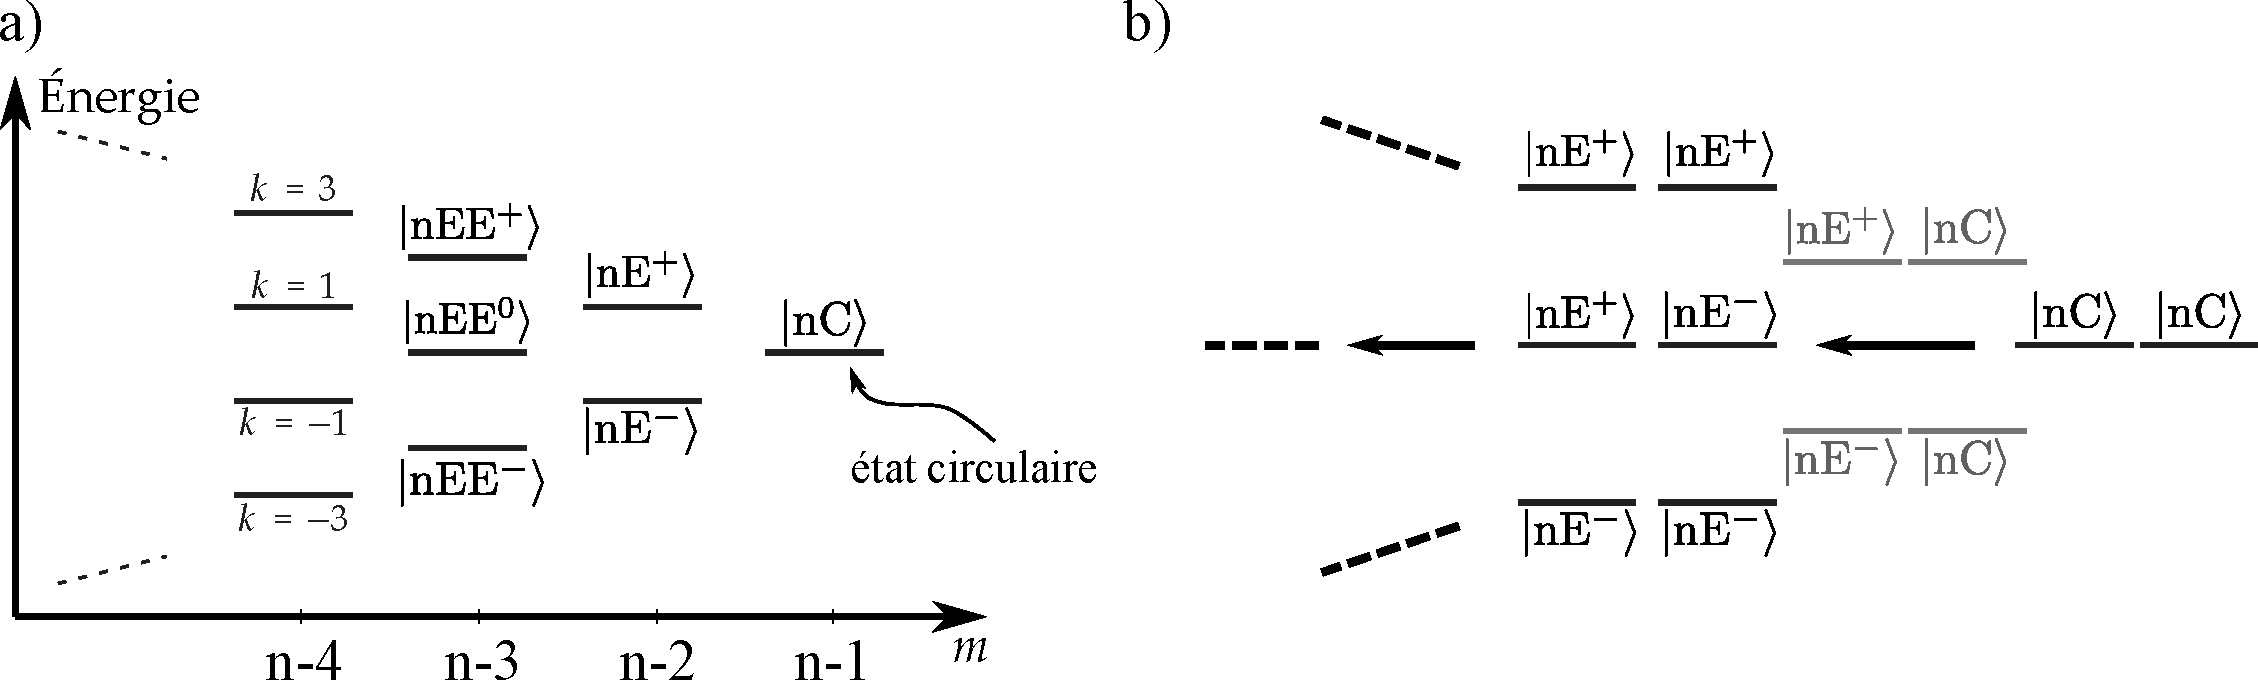
\includegraphics[width=\linewidth]{figures/circsim/diagram_nC_nCnC}
\caption[Diagammre d'énergie des niveaux proches du $\mathrm{50C}$]{
\textbf{a)} Diagramme d'énergie des niveaux proches de $\mathrm{nC}$, en présence d'un champ électrique.
\textbf{b)} Diagramme d'énergie des niveaux de paire proches de $\ket{\mathrm{nC}}\ket{\mathrm{nC}}$ en présence d'un champ électrique.
Le champ électrique est dirigé selon $Oz$, perpendiculaire au vecteur qui sépare les deux atomes de la paire,  dirigé selon $Ox$.
}
\label{fig:ener_StarknC_nCnC}
\end{figure}


Il s'agit maintenant de comprendre quelle forme prend l'interaction dipôle-dipôle dans le cas présent.
Replaçons nous dans le cas de deux atomes séparés d'une distance $r$.
En \ref{sec:interacting_rydbergs} nous avions exprimé, en l'absence de champ électrique extérieur, le hamiltonien de couplage dans la base des harmoniques sphériques (cf. équation \eqref{eq:Vdd_rr1r2}).
De plus, l'axe de quantification était alors déterminé par le vecteur séparant la paire d'atomes en interaction.
Ici au contraire, l'axe de quantification est déterminé par le champ électrique extérieur, selon $Oz$ donc, et les atomes sont situés sur l'axe $Ox$, à des positions $\vec{r_1},\vec{r_2}$ respectivement.
Le hamiltonien d'interaction dipôle-dipôle prend alors la forme
\begin{equation}
\label{eq:dipdip_nC}
\hat{V}_{dd} = -\frac{q^2\hat{r_1} \hat{r_2}}{3\epsilon_0 r^3}
\left[ Y_1^0 Y_1^0 + \frac{1}{2} \left( Y_1^{+1}Y_1^{-1} + Y_1^{-1}Y_1^{+1} \right)
- \frac{3}{2} \left(  Y_1^{+1}Y_1^{+1} + Y_1^{-1}Y_1^{-1} \right) \right],
\end{equation}
où les $Y_l^m$ sont les harmoniques sphériques.
On remarque ici que l'interaction dipôle-dipôle permet une variation du moment magnétique total de la paire atomique $\Delta M \leq 2$.
Ainsi le niveau de paire $\ket{\mathrm{nC},\mathrm{nC}}$ se trouve couplé de façon quasi-résonante avec les niveaux symétriques de paire dont l'énergie est suffisamment proche et dont le moment magnétique total est supérieur  à $2(n-2)$, tel que par exemple le niveau de paire $(\ket{\mathrm{nE^+},\mathrm{nE^-}}\pm\ket{\mathrm{nE^-},\mathrm{nE^+}})/\sqrt{2}$.
Ces niveaux sont à leur tour couplés au niveaux symétriques de paire proches en énergie et dont le moment magnétique total est supérieur à $2(n-2)$, tel que par exemple $\ket{\mathrm{nEE^0},\mathrm{nEE^0}}$.
La figure (\ref{fig:ener_StarknC_nCnC} b) représente les niveaux de paire proches du niveau $\ket{\mathrm{nC},\mathrm{nC}}$ en présence d'un champ électrique.

Ces couplages quasi-résonants, dès lors que la distance entre les atomes est suffisamment petite, perturbent le niveau $\ket{\mathrm{nC,nC}}$ en le mélangeant aux niveaux de paires d'énergie suffisamment proche.
C'est ce que nous avions vu en \ref{subsec:interac50C_I} : lorsque les deux atomes de la paire sont plus proches que $\SI{10}{\um}$, l'état propre du hamiltonien complet s'éloigne du niveau non perturbé $\ket{\mathrm{50C,50C}}$.
La figure (\ref{fig:VdW_50C50C_1Vcm_10G} a) reproduit la figure \eqref{fig:VdW_50C50C_1Vcm}, représentant l'énergie d'interaction d'une telle paire atomique en fonction de la distance entre les deux atomes.
On y voit la première conséquence néfaste de l'effet de mélange : l'interaction dipôle-dipôle entre deux atomes de Rydberg circulaires dans le même niveau ne peut plus être simplement représentée par un déplacement d'énergie en $1/r^6$ .
%Cet effet de mélange a plusieurs conséquences néfastes.
%Tout d'abord, l'interaction dipôle-dipôle ne peut plus être simplement représentée par un déplacement d'énergie en $1/r^6$ entre deux atomes dans un niveau de paire $\ket{n,m,k}\ket{n,m,k}$.
%De plus, le mélange avec les niveaux elliptiques réduit le temps de vie du niveau de paire à deux atomes circulaires.
%En effet, les niveaux elliptiques peuvent être deséxcités par des transitions $\pi$ vers la multiplicité inférieure alors que le niveau circulaire ne peut être deséxcité que par une transition $\sigma^+$.
%Or le dispositif d'inhibition de l'émission spontanée que nous proposons, discuté en \ref{subsec:inhibition}, ne peut inhiber que l'émission spontanée $\sigma^+$.
%Ainsi donc, le gain de temps de vie permis par ce dispositif est perdu dès lors que des transitions $\pi$ sont accessibles.

Afin de contourner cette difficulté, il faut trouver un moyen de lever la dégénérescence des niveaux de paire non perturbés représentés en figure (\ref{fig:ener_StarknC_nCnC} b).
Deux paramètres sont à notre disposition pour ce faire.
Le premier est la valeur du champ électrique.
Les niveaux de paire non perturbés sont d'autant plus distants en énergie que le champ électrique est élevé.
Cependant, la variation du champ électrique nous sert à faire varier l'interaction elle-même, comme nous l'expliquions en \ref{subsec:XXZhamiltonian}.
Le second moyen dont nous disposons est l'imposition d'un champ magnétique extérieur $B_z$, orienté selon $Oz$, qui déplacera les niveaux par effet Zeeman.

Le hamiltonien Zeeman pour un état circulaire prend la forme%\footnote{
%on néglige le spin de l'électron
%}
\begin{equation}
\label{eq:H_Zeeman}
\hat{H}_Z = \mu_B g_l~\hat{\vec{L}}\cdot\vec{B} = \mu_B g_l\hat{L}_zB_z,
%\frac{\mu_B g_l}{\hbar}~\hat{\vec{L}}\cdot\vec{B} = \frac{\mu_B g_l}{\hbar}\hat{L}_zB_z,
\end{equation}
où $\mu_B$ est le magnéton de Bohr et $g_l$ le facteur de Landé pour le nombre quantique orbital $l$.
Dans la mesure où l'on néglige le spin de l'électron, qui est très petit devant $l$ ($s=1/2 \ll l\simeq 50$), le facteur de Landé peut être approximé à $g_l \simeq 1$.
Ce hamiltonien conserve le nombre quantique magnétique $m$, qui n'est autre que la valeur propre de l'opérateur $\hat{L_z}$\footnote{
Si le champ magnétique avait des composantes non nulles selon $Ox$ et $Oy$, celles-ci coupleraient des états de $m$ différents.}.
Tant que le champ magnétique $B_z$ reste suffisamment petit, l'effet Zeeman agit comme une perturbation au premier ordre du hamiltonien \eqref{eq:hamilt_Stark} de l'atome dans un champ électrique.
La seule conséquence de l'effet Zeeman sur le niveau $\ket{n,m,k}$ sera alors un déplacement d'énergie
\begin{equation}
\label{eq:Zeeman_shift}
\Delta E_Z (n,m,k) = \braket{n,m,k|g_l \hat{L}_z | n,m,k}\cdot \mu_B B_z \simeq m\cdot \mu_B B_z = \Delta E_Z (m).
\end{equation}
Le niveau de paire $\ket{n,m,k ; n,m',k'}$ sera déplacé de la somme du déplacement d'énergie de $\ket{n,m,k}$ et $\ket{n,m',k'}$, soit $(m+m')\mu_B B_z$.

En tenant compte de l'effet Stark (cf. équation \eqref{eq:Stark_circular}) et de l'effet Zeeman perturbatif, on obtient les énergies suivantes pour les niveaux circulaires et elliptiques de la multiplicité $n$ :
\begin{equation}
\label{eq:ener_nC_ZeeStark}
\begin{aligned}
E_{\mathrm{nC}}/2E_I &= -\frac{1}{2n^2} - \frac{1}{16}n^4(8n^2+18n+10)|\vec{F}|^2 \left(\frac{ea_0}{2E_I} \right)^2 + (n-1)\mu_B B_z \\
&= -\frac{1}{2n^2} - \alpha_{\mathrm{nC}}|\vec{F}|^2 + (n-1)\mu_B B_z ,\\
E_{\mathrm{nE^{\pm}}}/2E_I &= -\frac{1}{2n^2} \pm \frac{3n}{2}|\vec{F}|\frac{ea_0}{2E_I} - \frac{1}{16}n^4(8n^2+36n-20)|\vec{F}|^2\left(\frac{ea_0}{2E_I} \right)^2 + (n-2)\mu_B B_z \\
&= -\frac{1}{2n^2} \pm \frac{ea_0}{2E_I}\frac{3n}{2}|\vec{F}| +\alpha_{\mathrm{nE^{\pm}}}|\vec{F}|^2 + (n-2)\mu_B B_z,
\end{aligned}
\end{equation}
où les coefficients $\alpha$ d'effet Stark quadratique sont introduits pour simplifier l'écriture et $E_I$ est l'énergie d'ionisation corrigée pour la masse du \Rb{87}.

Appliquons les équations \eqref{eq:ener_nC_ZeeStark} à l'exemple des états de paire non perturbés $\ket{\mathrm{50C,50C}}$ et $\ket{\mathrm{50E^+,50E^-}}$.
Dans les conditions du paragraphe \ref{subsec:interac50C_I}, c'est-à-dire sous $\SI{1}{\V/cm}$ et sans champ magnétique, la distance en énergie entre ces deux états de paire est de $\Delta_E = h\times\SI{169}{\kHz}$.
Si l'on ajoute un champ magnétique $B_z$ de $\SI{10}{\gauss}=\SI{1}{\milli\tesla}$, la distance en énergie devient $\Delta E = h\times \SI{28.17}{\MHz}$, soit presque $\SI{200}{}$ fois plus.
Un faible champ magnétique nous permet ainsi de lever la dégénérescence entre les niveaux de  paire voisins de $\ket{\mathrm{nC,nC}}$.

%\subsubsection*{L'interaction circulaire-circulaire en présence de champs électrique et magnétique extérieurs}
%\noindent Dans les conditions que nous venons d'établir il nous est possible de calculer l'interaction dipôle-dipôle entre deux atomes circulaires, tout en limitant la perturbation de ces niveaux qui serait due à un couplage résonant.
%Ce calcul s'effectue de la même façon qu'en \ref{sec:interacting_rydbergs}, en diagonalisant le hamiltonien complet de la paire atomique\footnote{
%La même méthode permet tout aussi bien de calculer l'interaction entre deux atomes dans des niveaux différents, de même qu'en \ref{sec:interacting_rydbergs}.
%}.
%Ce hamiltonien complet s'écrit
%\begin{equation}
%\label{eq:hamilt_Vdd_ZeeStark}
%\begin{aligned}
%\hat{H} &= \hat{H}_1 + \hat{H}_2 + \hat{V}_{dd}(\vec{r}) \\
% &= \hat{H}_{0,1} + \hat{H}_{0,2} + \hat{H}_{S,1} + \hat{H}_{S,2} + \hat{H}_{Z,1} + \hat{H}_{Z,2} + \hat{V}_{dd}(\vec{r}),
%\end{aligned}
%\end{equation}
%où $\hat{H}_{0,i},\hat{H}_{S,i},\hat{H}_{Z,i}$ sont respectivement les hamiltoniens libre, Stark et Zeeman de l'atome $i$ et $\hat{H}_i$ le hamiltonien total de l'atome $i$ isolé.
%
%Nous pouvons, ici encore, écrire l'interaction entre un atome dans le niveau $\mathrm{nC}$ et un atome dans le niveau $\mathrm{n'C}$ comme un hamiltonien effectif
%\begin{equation}
%\label{eq:Veff_nCn'C}
%V_{eff}/h = \left(\begin{array}{cc}
%C_{\mathrm{nC},\mathrm{n'C}} & A_{\mathrm{nC},\mathrm{n'C}} \\
%A_{\mathrm{nC},\mathrm{n'C}} & C_{\mathrm{nC},\mathrm{n'C}},
%\end{array} \right)
%\end{equation}
%où $C_{\mathrm{nC},\mathrm{n'C}}$ et $A_{\mathrm{nC},\mathrm{n'C}}$ sont respectivement les termes d'interaction directe et d'échange entre les niveaux $\mathrm{nC}$ et $\mathrm{n'C}$.
%De manière générale, ces termes se décomposent en une composante \og van der Waals \fg{} en $1/r^6$ et une composante de couplage direct en $1/r^3$.
%De plus, ils dépendent désormais fortement des champs électrique et magnétique imposés.

Reprenons l'exemple de deux atomes dans l'état $\ket{\mathrm{50C,50C}}$.
%Les deux atomes étant dans le même état, l'interaction se limitera aux termes diagonaux du hamiltonien \eqref{eq:Veff_nCn'C} et aucune interaction d'échange n'aura lieu.
%Dans le paragraphe \ref{subsec:interac50C_I}, sans champ magnétique extérieur et sous $\SI{1}{\V/\cm}$, le niveau de paire se mélangeait dès que la distance entre les deux atomes était inférieure à $\SI{10}{\um}$.
%Le résultat de ce calcul est à nouveau présenté en figure (\ref{fig:VdW_50C50C_1Vcm_10G} a).
En refaisant le calcul de l'interaction, cette fois avec un champ magnétique $B_z=\SI{10}{\gauss}$, on obtient la courbe d'énergie présentée en figure (\ref{fig:VdW_50C50C_1Vcm_10G} b).
%
\begin{figure}[h]
\centering
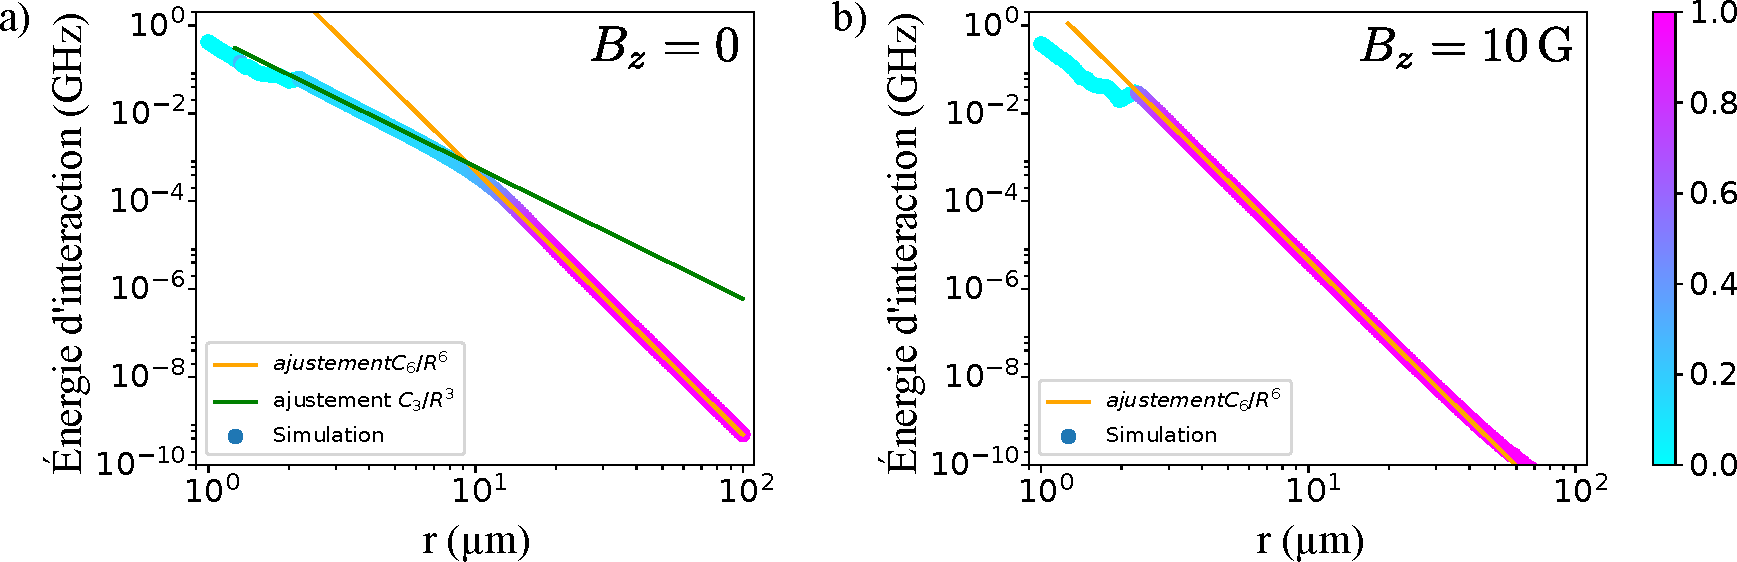
\includegraphics[width=\linewidth]{figures/circsim/VdW_50C50C_1Vcm_0_10G}
\caption[Interaction dipolaire 50C-50C en présence d'un champ magnétique]{
Déplacement en énergie de la paire 50C-50C par interaction dipolaire.
Les deux atomes sont placés côte à côte sur l'axe $Ox$, sous un champ électrique de $\SIvv{1}{\V / \cm}$ selon l'axe $Oz$. L'échelle de couleur, commune aux deux graphes, représente le carré de la projection sur l'état non perturbé $\ket{50\text{C},50\text{C}}$ de l'état propre du hamiltonien qui le suit adiabatiquement.
\textbf{a)} Sans champ magnétique extérieur et \textbf{b)} avec un champ magnétique $B_z = \SI{10}{\gauss}$ selon $Oz$.
}
\label{fig:VdW_50C50C_1Vcm_10G}
\end{figure}
%
Alors qu'en l'absence de champ magnétique le niveau de paire circulaire-circulaire était perturbé dès que la distance entre les deux atomes était inférieure à $\SI{10}{\um}$, un champ magnétique de $\SI{10}{\gauss}$ selon $Oz$ permet d'éviter cet effet.
L'énergie d'interaction évolue ainsi en $1/r^6$ pour les distances supérieures à $\SI{2}{\um}$.
Cependant, l'interaction est rendue moins forte.
En effet, un ajustement en $1/r^6$ donne un coefficient de van der Waals $C_{6,\mathrm{50C-50C}}(\SI{10}{\gauss}) = \SI{4.448}{\GHz\raiseto{6}\um}$ au lieu de $\SI{489.18}{\GHz\raiseto{6}\um}$ en champ magnétique nul.
Cela s'explique par le fait que le couplage dipolaire second de ordre varie comme l'inverse des distances en énergie entre le niveau de paire considéré et les niveaux médiateurs du couplage.
Le champ magnétique ayant pour effet de déplacer les niveaux de paire de façon à supprimer les couplages quasi résonants, il s'en suit que les distance en énergie entre niveaux de paire sont augmentées et l'interaction d'autant diminuée.
%
%Dans le cas d'une paire d'atomes dans l'état $\ket{\mathrm{nC,n'C}}$ avec $n'\neq n$, une interaction d'échange décrite par le coefficient $A_{\mathrm{nC},\mathrm{n'C}}$ aura lieu, en plus de l'interaction directe décrite par le coefficient $C_{\mathrm{nC},\mathrm{n'C}}$.
%La présence d'un champ magnétique permet, ici aussi, de lever les dégénérescences de niveaux qui induiraient une interaction d'échange de premier ordre, c'est-à-dire variant en $1/r^3$.

\subsection{Limitation du temps de vie des niveaux circulaires}

\noindent Dès lors que l'on presque supprimé le facteur principal limitant la durée de vie des niveaux de Rydberg, il devient nécessaire de prendre en compte des facteurs qui paraissaient auparavant négligeables.
Le plus important de ces effets est le mélange des niveaux de paire décrit ci-dessus.
En effet, les niveaux elliptiques $\mathrm{nE^{\pm}}$ peuvent se désexciter spontanément par d'autres transitions que le niveaux circulaire $\mathrm{nC}$, en particulier vers le niveau $\mathrm{(n-1)C}$ par une transition $\pi$ et vers le niveau $\mathrm{(n-2)C}$ par une transition $\sigma^+$ de plus petite longueur d'onde.
Aucune de ces deux transitions, représentées sur la figure \ref{fig:sigma_pi}, n'étant inhibée par le condensateur, il est essentiel pour la durée de vie de notre chaîne atomique de limiter le mélange des niveaux de paire.
Pour cela, il faudrait imposer de grands champs électrique et magnétique.
Les valeurs de ces champs doivent toutefois être limitées, car nous souhaitons conserver la possibilité de faire varier le paramètre d'interaction $J_z/J$.
La gamme de champs présentée en \ref{subsec:XXZhamiltonian}, de $\SI{2}{}$ à $\SI{12}{\V/\cm}$ pour le champ électrique et de $\SI{9}{}$ à $\SI{13}{\gauss}$ pour le champ électrique, est un bon compromis entre ces deux exigences.
\begin{figure}[h]
\centering
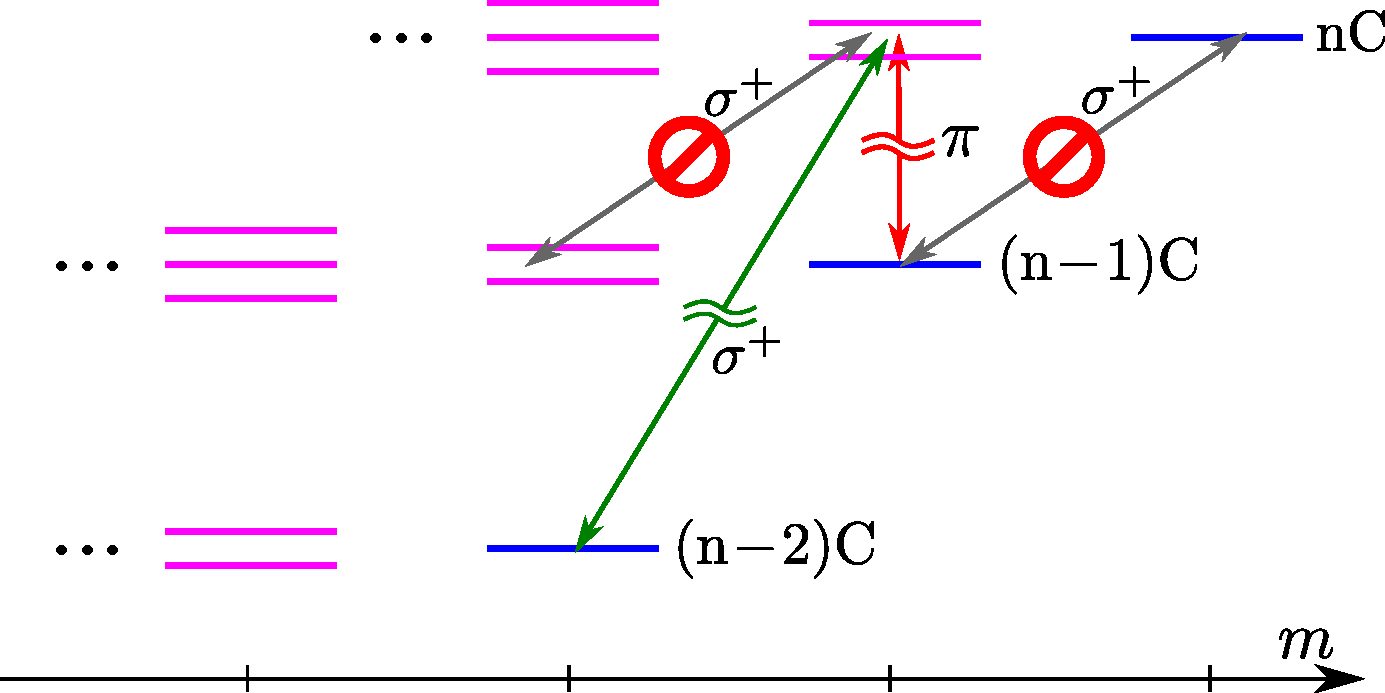
\includegraphics[width=0.7 \linewidth]{figures/circsim/sigma_pi}
\caption[Transitions spontanées depuis les niveaux elliptiques $\mathrm{nE^\pm}$]{
Transitions spontanées depuis le niveau circulaire $\mathrm{nC}$ et les niveaux elliptiques $\mathrm{nE^\pm}$.
Les transitions $\sigma^+$ de la multiplicité $n$ vers la multiplicité $n-1$ sont inhibées par le condensateur.
Les transitions $\pi$ et $\sigma^+$ depuis les niveaux $\mathrm{nE^\pm}$ vers les niveaux $\mathrm{(n-1)C}$ et $\mathrm{(n-2)C}$ respectivement ne sont pas inhibées.
}
\label{fig:sigma_pi}
\end{figure}

D'autres effets viennent réduire la durée de vie des atomes de Rydberg piégés. % : la présence de photons thermiques à température finie, les collisions avec le gaz résiduel,  la photo-ionisation due au laser de piégeage ainsi que la diffusion élastique des photons de ce même laser.
%
En premier lieu, la température finie de l'environnement induit des photons thermiques dans le domaine microonde, qui stimulent la transition $\pi$ depuis le niveau $\mathrm{nC}$ vers l'un des deux niveaux elliptiques $\mathrm{(n+1)E^\pm}$ de la multiplicité du dessus.
Or ces transitions ne sont pas inhibées par le condensateur.
Au contraire, elles sont favorisées par le grand nombre de modes électromagnétiques qui peuvent se propager entre les deux plaques et parallèlement à celles-ci.
Le taux d'émission de ces transitions est augmenté d'un facteur $\approx \SI{2}{}$.
Il est donc important de refroidir l'environnement expérimental le mieux possible, et nous proposons une température de $\SI{0.4}{\K}$, accessible avec un cryostat à $^3$He sans dilution.

Un facteur supplémentaire de réduction de la durée de vie provient des collisions des atomes avec le gaz résiduel dans l'enceinte à vide.
En environnement cryogénique, des pressions de l'ordre de $\SI{e-14}{\milli\bar}$ sont accessibles sans trop de difficulté \cite{MX_GABRIELSEANTIPROTON90,MX_WERTHCRYOION98}, limitant cet effet.

La photo-ionisation des atomes de Rydberg due au laser de piégeage doit aussi être prise en compte.
Heureusement, cet effet reste petit pour les niveaux circulaires, en raison du mauvais recouvrement entre leur fonction d'onde et les fonctions d'onde des électrons dans le continuum
\footnote{Les fonctions d'onde électroniques dans le continuum oscillent rapidement, alors que la fonction d'onde de l'électron dans un niveau circulaire varie lentement avec la distance au noyau.}.

Les photons du laser de piégeage peuvent également être élastiquement diffusés par les électrons de Rydberg. L'électron recevrait alors une importante quantité de mouvement pouvant induire une transition vers un niveau elliptique.
La contribution de cet effet peut être calculée dans un modèle classique de diffusion Thomson.

Enfin, les processus de relaxation dipolaire peuvent également limiter la durée de vie : une paire d'atomes dans le niveau $\ket{\mathrm{nC,nC}}$ est transférée dans le niveau de paire $\ket{\mathrm{nE^- , nE^-}}$, et l'énergie libérée par cette transition est convertie en énergie cinétique. Les deux atomes elliptiques concernés seraient alors expulsés à grande vitesse.
Cependant, l'élément de matrice de transition entre l'état initial piégé et l'état final, qui est une onde plane d'énergie élevée, est faible.


Les contributions de chacun de ces effets sont discutées dans la thèse de Thanh Long Nguyen \cite{PHD_NGUYEN} et dans \cite{ENS_PRE_CIRCSIM}.
Le tableau \ref{tab:lifetime_circsim} en fait la synthèse
%
\begin{table}[!h]
	\centering
	\caption[Contributions des différents effets limitant le temps de vie des atomes circulaires]{Contributions des différents effets limitant le temps de vie des atomes circulaires, pour une paire d'atomes dans le niveau $\mathrm{48C}$, séparés d'une distance $d=\SI{5}{\um}$, sous un champ électrique $F=\SI{6}{\V/\cm}$ et un champ magnétique $B_z=\SI{13}{\gauss}$.
	Les atomes sont placés dans un condensateur de taille $a=\SI{13}{\mm}$ et d'écartement $D=\SI{2}{\mm}$ et l'environnement est refroidi à $\SI{0.4}{\K}$ sous une pression de $\SI{e-14}{\milli\bar}$.
	}
	\label{tab:lifetime_circsim}
	\begin{tabular}{c c}
		\toprule\midrule
		Phénomène
		& Temps de vie (\si{\second})\\
		\midrule
		Émission spontanée résiduelle & \SI{2500}{} \\
		Émission stimulée par rayonnement du corps noir & \SI{630}{} \\
		Collisions avec le gaz résiduel à $\SI{e-14}{\milli\bar}$ & \SI{400}{} \\
		Photo-ionisation & $\infty$ \\
		Diffusion élastique des photons du piège & \SI{> 180}{} \\
		Relaxation dipolaire & $\infty$ \\
		Mélange des niveaux de paire & \SI{88}{} \\
		\midrule \midrule
		Temps de vie total & 47 \\
		\midrule \bottomrule
 	\end{tabular}
\end{table}
%
En tenant compte de tous ces effets, nous estimons la durée de vie d'un atome individuel à $\SI{47}{\second}$.
La durée de vie d'une chaîne de $\SI{40}{}$ atomes est alors supérieure à la seconde.
Cette borne inférieure est vérifiée dans l'ensemble du domaine de champs électrique et magnétique représenté en figure \ref{fig:Jz_Jscan} permettant le contrôle du paramètre $J_z/J$.
Cette durée de vie supérieure à une seconde représente de l'ordre de $\SI{80000}{}$ temps d'échange $\tau_{\text{éch}}$ à $d=\SI{5}{\um}$.
Le simulateur quantique pourra ainsi évoluer sur des temps très longs et permettre d'observer des dynamiques lentes telles que des rétablissements d'équilibre ou des processus de thermalisation.

%	\subsection{Préparation déterministe d'une chaîne}\label{subsec:vdW_evap}
%\noindent À des fins évidentes de reproductibilité, la chaîne de $N$ atomes constituant le simulateur doit être préparée de façon déterministe.
%Pour cela, nous proposons une méthode de préparation fondée sur une variante du refroidissement évaporatif.
%Une chaîne initiale, irrégulière et contenant un grand nombre aléatoire d'atomes, est comprimée et \og évaporée \fg{} jusqu'à obtenir le nombre d'atomes et la distance inter-atomique souhaités.
%Ce processus d'évaporation refroidit les atomes presque jusqu'à l'état fondamental du piège laser.
%Cette technique permet également d'obtenir une détection individuelle des atomes de Rydberg.
%
%Une séquence expérimentale typique commence par la préparation d'un nuage thermique de \Rb{87} près d'une puce supraconductrice, très allongé dans la direction $x$ et refroidi à une température inférieure à $\SI{1}{\uK}$, proche de la dégénérescence.
%Ce nuage est ensuite piégé dans un faisceau laser focalisé et déplacé vers le condensateur d'inhibition précédemment décrit.
%Là, après extinction du piège dipolaire, une impulsion laser à deux photons excite un nuage d'atomes de Rydberg à bas moment cinétique dans le niveau $n=50$, en régime de blocage dipolaire.
%En raison de la forme allongée du nuage d'atomes dans l'état fondamental et du blocage dipolaire, cet ensemble d'atomes de Rydberg est une chaîne irrégulière contenant une centaine d'atomes distants de $\SI{9}{}\pm\SI{3}{\um}$.
%Les atomes dans l'état fondamental sont expulsés par une impulsion laser résonante à $\SI{780}{\nano\meter}$ , et les atomes de Rydberg sont transférés vers l'état circulaire $\mathrm{50C}$ grâce à un champ radio-fréquence polarisé $\sigma^+$\footnote{Le processus de circularisation sera discuté au chapitre \ref{chapter:50c}.}.
%
%Lorsque les atomes de Rydberg circulaires sont excités, le faisceau Laguerre-Gauss de confinement radial est allumé, en même temps que deux faisceaux gaussiens \og bouchons \fg{} parallèles à l'axe $Oy$.
%Ces deux faisceaux à $\SI{1064}{\nano\meter}$ créent deux barrières d'énergie sur l'axe $Ox$, centrées en $x=\pm L/2$, représentées en figure (\ref{fig:plugs_evap} a).
%Le bouchon de droite ($x=+L/2$) est plus bas en énergie que celui de gauche.
%Le piège est ensuite comprimé en réduisant $L$.
%Ce faisant, les atomes de Rydberg sont approchés les uns des autres ce qui fait augmenter l'interaction répulsive de van der Waals.
%Lorsque la chaîne d'atomes est suffisamment comprimée, l'atome en bout de chaîne à droite a une énergie d'interaction qui devient supérieure à la hauteur de la barrière créée par le bouchon laser, et cet atome est ainsi éjecté de la chaîne, comme cela est représenté en figure (\ref{fig:plugs_evap} b).
%Les atomes restants se redistribuent selon l'axe $x$ et l'énergie totale de la chaîne se trouve diminuée par cette \og évaporation \fg{} d'un atome.
%Le nombre final d'atomes dans la chaîne est déterminé par la valeur finale de $L$ et par la hauteur en énergie du bouchon laser.
%%
%\begin{figure}[h]
%\centering
%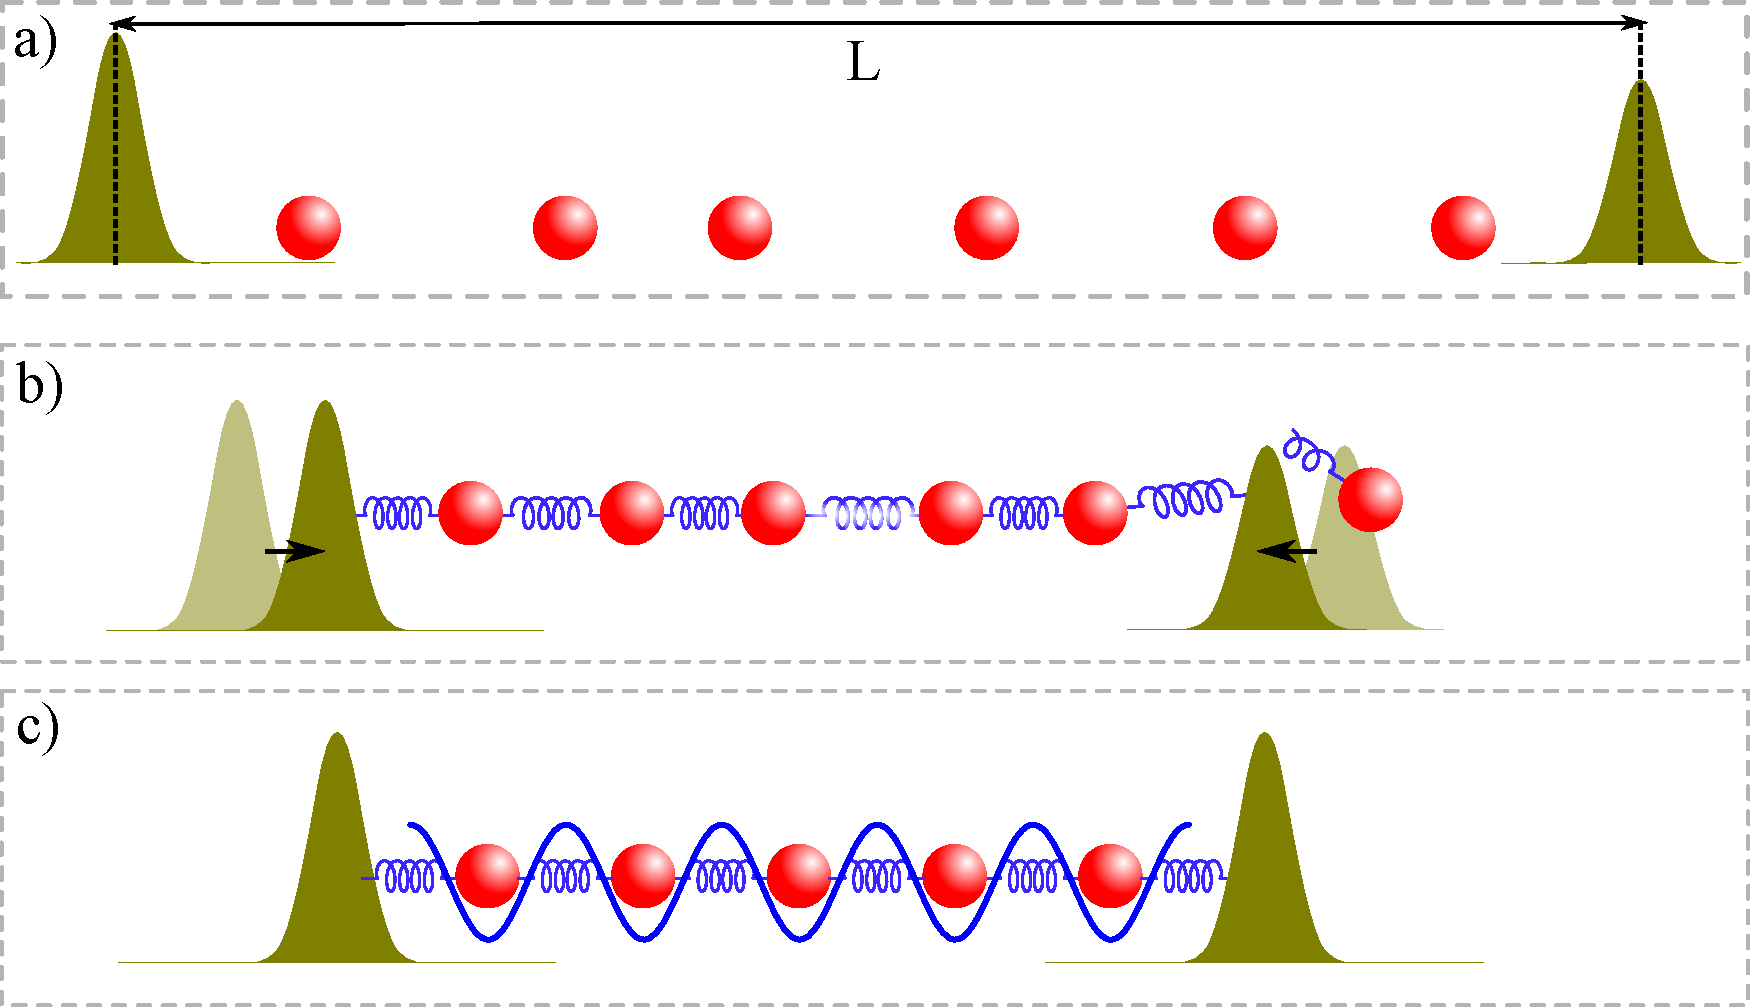
\includegraphics[width=0.8\linewidth]{figures/circsim/plugs_evap}
%\caption[Schéma de l'\og evaporation van der Waals \fg{} ]{
%Schéma de l'\og evaporation van der Waals \fg{}.
%\textbf{a)} Une chaîne irrégulière est préparée et piégée entre deux \og bouchons \fg{} laser spéarés d'une distance $L$.
%\textbf{b)} En diminuant $L$, on augmente les interactions de van der Waals répulsives entre les atomes de la chaîne.
%La barrière énergétique étant plus basse à droite, l'atome au bout de la chaîne est éjecté.
%\textbf{c)} \`A la fin du processus d'évaporation, on obtient de façon déterministe une chaîne régulière de $N$ atomes. Un réseau laser est allumé afin de piéger chaque atome.
%}
%\label{fig:plugs_evap}
%\end{figure}
%%
%
%Ce processus de refroidissement évaporatif peut être simulé numériquement de façon quasi-classique.
%La figure \eqref{fig:nevap} présente le résultat de $\SI{100}{}$ réalisations de la séquence d'évaporation, en moyenne et variance du nombre d'atomes final en fonction de la valeur finale de $L$.
%Pour les nombres d'atomes inférieurs à $\SI{45}{}$, $N$ évolue par des pas bien définis, et l'insert qui détaille les résultats autour de $N=40$ montre l'annulation de la variance du nombre d'atomes à certaines valeurs de $L$.
%En arrêtant à ces longueurs de piège le processus d'évaporation, nous obtenons de façon déterministe une chaîne avec le nombre d'atomes voulu.
%La distance inter-atomique $d$ est ensuite choisie par un ajustement fin de la longueur $L$.
%%
%\begin{figure}[h]
%\centering
%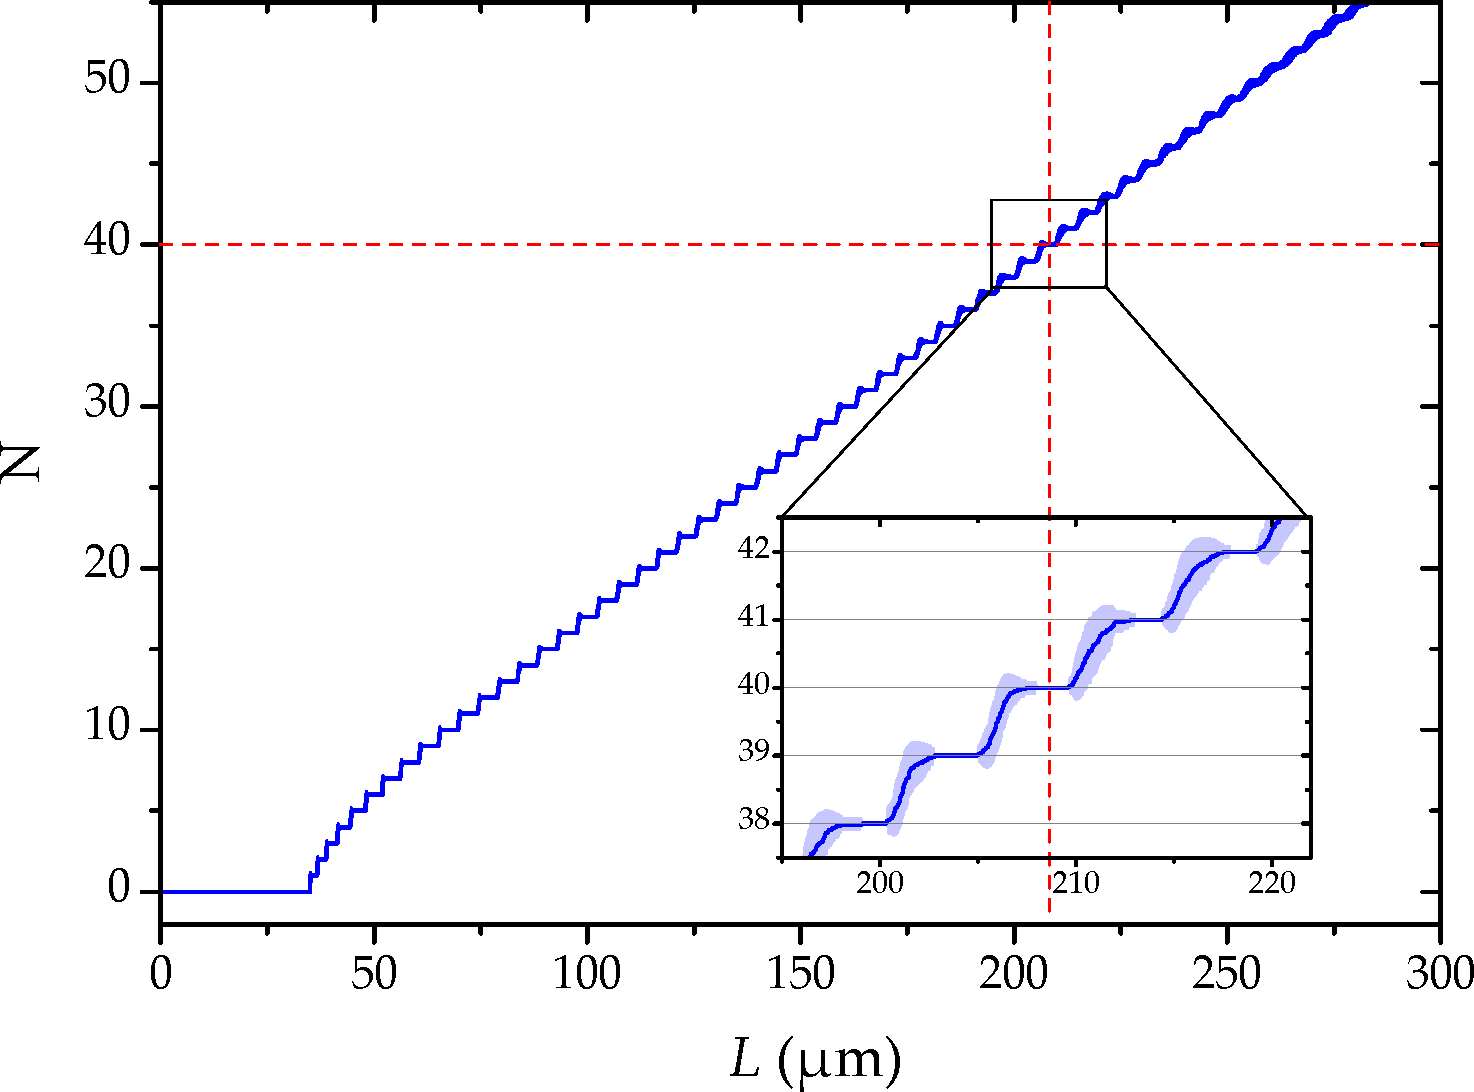
\includegraphics[width=0.6\linewidth]{figures/circsim/nevap}
%\caption[Nombre d'atomes restant après évaporation van der Waals]{
%Nombre d'atomes $N$ restant après l'évaporation van der Waals, en fonction de la valeur finale de la distance $L$ entre les deux bouchons laser.
%Le trait plein représente la moyenne de $N$ sur $100$ réalisations du processus d'évaporation.
%La variance de $N$ est indiquée par les zones bleu clair.
%
%}
%\label{fig:nevap}
%\end{figure}
%%
%
%Enfin, le réseau laser de confinement longitudinal est allumé adiabatiquement afin de fixer les positions atomiques.
%Les faisceaux bouchons sont gardés allumés, avec une puissance ajustée de façon à compenser la répulsion des atomes du bout de la chaîne par leur unique voisin.
%L'état final de la chaîne d'atomes est représenté en figure (\ref{fig:plugs_evap} c).
%
%La procédure d'évaporation peut également servir à la détection des atomes de Rydberg.
%\`A la fin de l'évolution de la chaîne de spins, une impulsion $\pi$ microonde est appliquée sur la transition $\mathrm{48C}\rightarrow\mathrm{46C}$.
%Si elle présente une fréquence de Rabi suffisante, cette impulsion assure le transfert vers le niveau $\mathrm{46C}$ de tous les atomes dans le niveau $\mathrm{48C}$, quelle que soit leur énergie d'interaction.
%L'interaction d'échange entre $\mathrm{50C}-\mathrm{46C}$ étant de l'ordre du $\SI{}{\milli\hertz}$, ce transfert arrête l'évolution de la chaîne de spins et \og gèle \fg{} les états de spin.
%Le réseau de confinement longitudinal est alors éteint, et le processus d'évaporation par compression de la chaîne peut reprendre.
%Chaque atome est ainsi tour à tour expulsé de la chaîne et guidé par le faisceau Laguerre-Gauss vers une zone de détection située en-dehors du condensateur d'inhibition.
%Ils sont détectés dans cette zone par ionisation, ce qui projette leur état sur la base $\{\ket{\mathrm{46C}},\ket{\mathrm{50C}}\}$, équivalente à la base $\{\ket{\uparrow},\ket{\downarrow} \}$.
%Grâce à une impulsion microonde supplémentaire, appliquée juste avant le gel des interactions, nous pouvons imposer une rotation arbitraire aux états de spin. Ainsi nous pouvons mesurer toute observable de spin souhaitée, la seule contrainte étant que cette observable doit être la même pour tous les atomes de la chaîne.
%En fin de compte, l'état de chaque spin peut être individuellement mesuré en fonction du temps selon n'importe quelle observable.
%Cela permet d'accéder à des fonctions de corrélations complexes et aux propriétés d'intrication de la chaîne de spins.

\section*{Conclusion}
\noindent Dans ce chapitre, nous avons développé une proposition expérimentale complète pour un simulateur quantique constitué d'atomes de Rydberg circulaires en interaction.
La méthode d'\og évaporation van der Waals \fg{} permet de préparer de façon déterministe une chaîne régulière d'une quarantaine d'atomes distants de $\SI{5}{\um}$.
Cette chaîne atomique est piégée dans un potentiel laser périodique, avec une durée de vie supérieure à la seconde grâce à l'inhibition de l'émission spontanée par un condensateur.

Les interactions dipôle-dipôle entre les niveaux de Rydberg circulaires $\mathrm{48C}$ et $\mathrm{50C}$ nous permettent de simuler le hamiltonien XXZ d'une chaîne de spins $1/2$.
Les paramètres de ce hamiltonien peuvent être contrôlés à l'envi, en variant les champs électrique et magnétique imposés aux atomes ainsi que la puissance et la fréquence d'une source microonde classique.
Ce contrôle des paramètres peut être fait très rapidement par rapport au temps caractéristique d'évolution $\tau_{\text{\'ech}} = \SI{14.7}{\us}$.

Enfin, les atomes constituant la chaîne de spins peuvent être détectés un par un.
La détection par ionisation distingue les différents niveaux de Rydberg, ce qui permet de mesurer toute observable de spin sur l'ensemble de la chaîne.

Un tel simulateur, d'une grande flexibilité, permettrait ainsi de simuler une chaîne de $\SI{40}{}$ spins $1/2$ en interaction, sur des échelles de temps de $\SIrange{e4}{e5}{}$ fois le temps caractéristique d'échange.















